%% thesis.tex 2014/04/11
%
% Based on sample files of unknown authorship.
%
% The Current Maintainer of this work is Paul Vojta.

\documentclass{ucbthesis}
\usepackage{biblatex}
\usepackage{amsmath, amssymb}
\usepackage[utf8]{inputenc}
\usepackage{graphicx}
\usepackage[margin=1in]{geometry}
\usepackage{deluxetable}

\newcommand{\lcdm}{$\texrm{\Lambda}$CDM}

% To compile this file, run "latex thesis", then "biber thesis"
% (or "bibtex thesis", if the output from latex asks for that instead),
% and then "latex thesis" (without the quotes in each case).

% Double spacing, if you want it.  Do not use for the final copy.
% \def\dsp{\def\baselinestretch{2.0}\large\normalsize}
% \dsp

% If the Grad. Division insists that the first paragraph of a section
% be indented (like the others), then include this line:
% \usepackage{indentfirst}

\bibliography{references}

\begin{document}

% Declarations for Front Matter

\title{Empirical Models of Type Ia Supernovae: Applications for Next-Generation Cosmological Surveys}
\author{Samantha Dixon}
\degreesemester{Summer}
\degreeyear{2020}
\degree{Doctor of Philosophy}
\chair{Professor Saul Perlmutter}
\othermembers{Professor Daniel Kasen \\
  Assistant Professor Fernando Perez}
\numberofmembers{3}
% Previous degrees are no longer to be listed on the title page.
% \prevdegrees{B.A. (University of Northern South Dakota at Hoople) 1978 \\
%   M.S. (Ed's School of Quantum Mechanics and Muffler Repair) 1989}
\field{Physics}
% Designated Emphasis -- this is optional, and rare
% \emphasis{Colloidal Telemetry}
% This is optional, and rare
% \jointinstitution{University of Western Maryland}
% This is optional
\campus{Berkeley}

% For a masters thesis, replace the above \documentclass line with
% \documentclass[masters]{ucbthesis}
% This affects the title and approval pages, which by default calls this
% document a "dissertation", not a "thesis".

\maketitle
% Delete (or comment out) the \approvalpage line for the final version.
\approvalpage
\copyrightpage

\begin{abstract}
Type Ia supernovae (SNe Ia) remain one of the best astronomical tools available for measuring large distances. Observations of SNe Ia were instrumental in the discovery of the accelerating expansion of the universe, and will be key to understanding the nature of the ``dark energy" driving this accelerating expansion. Surveys like LSST and the Roman Space Telescope supernova survey are currently being designed to discover and follow a large number of SNe Ia -- a large enough number that the statistical error will be far subdominant to the systematic error. In order to avoid biases in the cosmological parameters constrained by these future surveys, it is essential that we understand the sources and effects of systematic uncertainties. This dissertation addresses some of these systematic biases. 

In Chapter 2, we present two measurements of the extent of charge transfer inefficiency (CTI) in the detectors of the SNIFS instrument that was used to collect much of the data used throughout this dissertation. If the inefficiency is too high in spectroscopic instruments like SNIFS, the smearing that CTI causes can lead to misinterpretation of the resulting spectra. We find that the CTI is low in all detectors (about 1 photoelectron in every million is trapped), and that the low CTI remains stable over time.

Chapter 3 focuses on modeling a particular spectral region of Type Ia supernova spectra near maximum brightness. This region of the spectrum is used in some subclassification schemes of SNe Ia, and can also serve as a proxy for identifying changes in the populations of these subtypes with redshift. Our model can provide accurate measurements of ejecta velocities and the feature equivalent width using low-resolution and/or noisy spectra. Being able to use lower-quality spectra allows us to mitigate bias out to earlier eras of cosmic history by allowing us to monitor population drifts at higher redshifts.

In Chapter 4, we study two empirical models of Type Ia supernova spectral evolution (SALT2 and SNEMO) and measure how well they can capture a variety of near-maximum spectroscopic features. Our goal is to analyse how linear spectral models with differing number of parameters can capture non-linear features like ejecta velocities. In addition, we present a model for producing realistic mock spectra based on these models, allowing future studies to have access to spectral templates that capture the full range of supernova spectral behavior.

Chapter 5 centers on an assumption of linear regression that is often overlooked in supernova cosmology analyses. These analyses perform an initial linear regression to correct the observed SN absolute magnitudes for other properties of the SN. They then perform a second regression to correct the residuals of this first regression for an additional covariate. This practice is statistically sound only if the covariates in the initial regression are not correlated with the covariates used in the second regression. However, these correlations do exist. We present a toy model of this problem to calculate closed-form expressions and scaling relations of the size of the biases in the effect sizes and estimated scatter that come from this overlooked assumption. We also use simulations based on literature data to calculate the size of these biases and provide potential corrections.

Chapter 6 presents two new models of Type Ia supernova spectroscopy that were constructed using deep learning. These models extend the ``twins embedding" model of Boone et al. (submitted) into a wide range of phases. The \texttt{spec2embed} model takes as input a spectrum observed at any phase from -10 to +40 days after maximum brightness, and predicts the spectrum's phase and its supernova's location in the twins embedding space. Using these predictions, we can standardize supernovae from single spectra with comparable precision to the original twins embedding work. The \texttt{embed2spec} model works in reverse, taking a phase (or range of phases) and location in the twins embedding space to predict a spectrum. With this, we can use forward-modeling fitting techniques to constrain a supernova's location in the twins embedding space from multiple spectra, spectra with lower spectral resolution, or even broadband photometry.
\end{abstract}

\begin{frontmatter}

\begin{dedication}
\null\vfil
\begin{center}
To TBD \\\vspace{12pt}
For something I don't know yet
\end{center}
\vfil\null
\end{dedication}

% You can delete the \clearpage lines if you don't want these to start on
% separate pages.

\tableofcontents
\clearpage
\listoffigures
\clearpage
\listoftables

\begin{acknowledgements}
\begin{itemize}
    \item Thesis advisor: Saul Perlmutter
    \item Committee members: Bill Holzapfel (qual committee chair), Dan Kasen, Fernando Perez (filled in last minute)
    \item Senior mentors: Greg Aldering, Alex Kim
    \item Undergraduate mentors: Paolo Privitera, Al Kogut
    \item Lab mates: Kyle Boone, Kara Ponder, Ravi Gupta, Clare Saunders, Aleks Cikota, Brian Hayden
    \item Collaborators: David Rubin, Ben Rose, Rebekah Hounsell, Yu Ma
    \item Square: Deeksha Chugh, Zaki Ali, Morag Scrimgeour, Stephane Fotso, Jackie Brosamer
    \item GDSO: Mike Fang, Sumayah Rahman, James Arnemann
    \item Friends: Jeffrey Epstein, Jennet Dickinson, Tom Zick, Jessica Avva, Abi Polin
    \item Family: Parents Lisa and Fred, brother Jim, grandmother Carol
\end{itemize}

\end{acknowledgements}

\end{frontmatter}

\pagestyle{headings}

\chapter{Introduction}

\section{Expansion History of the Universe}
Cosmology is the study of the origin, evolution, and eventual fate of the Universe. The current standard model of cosmology, the LCDM \ model, posits that the Universe is governed by Einstein's equations of relativity with a cosmological constant $\textrm{Lambda}$ and cold dark matter. 

Einstein's field equations (including a cosmological constant) are
\begin{equation}
    G_{\mu\nu} + \Lambda g_{\mu\nu} = \frac{8\pi G}{c^4}T_{\mu\nu}
    \label{eq:einstein_field}
\end{equation}
Under this model, we use the Friedmann-Lema\^{i}tre-Robertson-Walker (FLRW) metric to encode the homogeneous, isotropic, and time-dependent expansion of space:
\begin{equation}
    -c^2 d\tau^2 = -c^2dt^2 + a(t)^2\left[dr^2 + S_k(r)d\Omega^2\right]
    \label{eq:flrw_metric}
\end{equation}
where
\begin{equation}
    S_k(r) =
    \begin{cases}
    R\sin(r/R) & k=+1\\
    r & k=0\\
    R\sinh(r/R) & k=-1
    \end{cases}
    \label{eq:curvature}
\end{equation}

All of the time-dependence is captured by the evolution of the scale factor $a$. With this metric, we can find the following analytic solution to Einstein's field equations:
\begin{align}
    \left(\frac{\dot{a}}{a}\right)^2 & = \frac{8\pi G}{3} \rho - \frac{kc^2}{a^2} + \frac{\Lambda c^2}{3}\\
    \frac{\ddot{a}}{a} & = -\frac{4\pi G}{3}\left(\rho + \frac{3p}{c^2}\right) + \frac{\Lambda c^2}{3}
    \label{eqn:friedmann_eqns}
\end{align}
where $k$ is the curvature, $\rho$ is the density and $p$ is the pressure. These are known as the Friedmann equations. The Hubble parameter $H$ is defined at By defining a critical density
\begin{equation}
    \rho_c = \frac{3H^2}{8\pi G}
\end{equation}
we can then 

\section{Supernova Cosmology}
The focus of the studies presented here are on improving our understanding of Type Ia supernovae as tools for measuring cosmological distances. Type Ia supernovae were believed to 

\section{SNIFS: the SuperNova Integral Field Spectrograph}
The vast majority of the data analyzed in this thesis was collected using the SuperNova Integral Field Spectrograph (SNIFS) by members of the Nearby Supernova Factory (SNfactory) collaboration. SNIFS is mounted 

\section{Empirical Models of Type Ia Supernovae}

\section{Summary}

\chapter{Measurements of Charge Transfer Efficiency in the SNIFS Detectors}
\label{chap:cte}

\section{Introduction}
Charge-coupled devices (CCDs) are ubiquitous in optical and infrared astronomy. Incident photons generate electrons in the bulk silicon of the CCD, and these photoelectrons are collected by a grid of pixels arranged on a series of parallel readout registers. By manipulating the voltages along the gates of these registers, we can shift the collected charge row-by-row into a second (serial) register. Similar voltage manipulations of the serial register create a signal that can be amplified and digitized. The charge shuffling alternates between the parallel and serial registers until all pixels have been read out and the image is reconstructed in software from the resulting signal.

Ideally, 100\% of the charge in each pixel would be transferred to the next pixel at each readout step. However, traps in the silicon lattice of the CCD can capture charge only to release it at a later time. The trapped and released charge leads to smearing of point sources along the direction of charge transfer and impedes our ability to get accurate photon counts. The magnitude of this effect is quantified by the charge transfer efficiency (CTE) of the CCD, defined as the fraction of charge that survives each pixel transfer. Because most of the CCDs used in astronomical applications make many transfers in each image (as they have thousands of pixels in each register), the CTE must be very close to unity, with typical values being around $1-10^{-6}$. Additionally, because a larger number of transfers results in a higher likelihood of encountering more traps, pixels that are further from the readout register are more effected by charge trapping. This effect is especially problematic for spectroscopic instruments since the increased smearing with distance to the amplifier can lead to effects like uneven broadening of spectral features.

In this work, we quantify the charge transfer efficiency of the CCDs in all channels (photometric, and blue and red spectroscopic) of the SuperNova Integral Field Spectrograph (SNIFS) using two methods. The initial characterization was done by first exposing the CCDs to a Fe-55 x-ray source in order to generate single-pixel events with a known energy spectrum and then measuring the photoelectron loss. Later, we performed a similar analysis using cosmic ray events extracted from the dark frames taken during each observing run, enabling in-situ measurements of the CTE.

\section{Initial Characterization with Fe-55 X-rays}
The standard method for measuring CTE involves exposing the CCD to photons with a known spectrum \cite{janesick_scientific_2001}. These photons generate single-pixel events in the CCD image with a known amount of charge. By plotting the amount of charge measured in each event as a function of the row number, we can quantify the extent of charge trapping by measuring the decrease in charge with distance from the amplifier. A common source for these characterizations is Fe-55, which produces strong lines from K-alpha and K-beta emission at 5.9 keV and 6.2 keV. These emission lines corresponding to photoelectron signals in the CCD of 1620 $\textrm{e}^-$ and 1778 $\textrm{e}^-$, respectively.

 We performed this characterization by exposing each of the SNIFS CCDs to a Fe-55 source. Using \verb|sep|, a Python implementation of the commonly-used \verb|SExtractor| package, we selected all events in the resulting images that had signal levels $>5\sigma$ above the background signal level. We then fit the histogram of digitized counts in these extracted events, $s(f)$, to a model of the Fe-55 spectrum:
\begin{equation}
    s = A_1 \exp\left(-\frac{(f-1620/g)^2}{2\sigma_1^2}\right) + A_2 \exp\left(-\frac{(f-1778/g)^2}{2\sigma_2^2}\right).
\end{equation}
This fit is done in order to measure the gain, $g$, of the CCD amplifier, allowing us to convert from ADU counts to electrons. The relative fraction of events from the K-alpha and K-beta emission (i.e. $A_1/A_2$), as well as the width of the emission lines are allowed to float, treating these quantities as nuisance parameters in the fit.

\begin{figure}
    \centering
    \includegraphics{figures/cte/spectrum_fit.pdf}
    \caption{Example spectrum of the Fe-55 X-rays events extracted from a single amplifier frame along with the best-fit model. The results of this fit are used to determine the amplifier gain from each frame.}
    \label{fig:xray_spectrum}
\end{figure}

We combined the events from several images per channel (22 for the blue channel, 26 for the red channel, and 8 for the photometric channel), using the gain measured from the spectrum fit for each image to convert the flux from ADU counts to number of electrons $N_{e^-}$. We select the events that correspond to K-alpha emission by choosing events with $1550 < N_{e^-} < 1700$. We then plot the flux for each event as a function of distance from the amplifier, shown in Fig. \ref{fig:cte_xray} for the parallel registers and Fig. \ref{fig:cte_xray_serial} for the serial register. The slope of the best-fit line (in units of $e^-$ per transfer), divided by the expected number of electrons (1620), gives us our measurement of the charge transfer inefficiency, or what fraction of charge is lost in each transfer. The resulting measurements of the charge transfer inefficiency are shown as labels in Figs. \ref{fig:cte_xray} and \ref{fig:cte_xray_serial}, as well as in Table \ref{tab:cte_xray}.

\begin{figure}[htbp]
    \centering
    \includegraphics[width=0.85\textwidth]{figures/cte/xray_cte_parallel.png}
    \caption{The number of electrons in extracted Fe-55 X-ray events as a function of y-location on the CCD for each camera amplifier (equivalent to number of transfers in the parallel direction). The slope of the best-fit line divided by the expected number of electrons gives us an estimate of the charge transfer inefficiency in the parallel registers.}
    \label{fig:cte_xray}
\end{figure}

\begin{figure}[htbp]
    \centering
    \includegraphics[width=0.85\textwidth]{figures/cte/xray_cte_serial.png}
    \caption{Same as Fig. \ref{fig:cte_xray}, but for the x-location of events. The best-fit lines are used to estimate the charge transfer inefficiency in the serial registers.}
    \label{fig:cte_xray_serial}
\end{figure}

\begin{table}[htbp]
    \centering
    \begin{tabular}{cccccc}\toprule
        Camera & Amp. & Parallel CTI & Serial CTI & Number of frames & Number of events \\\midrule
        B & A &0.783 $\;\pm\;$ 0.015 & 6.80 $\;\pm\;$ 0.03 & 22 & 15,925 \\
          & B &1.519 $\;\pm\;$ 0.017 & 3.14 $\;\pm\;$ 0.03 &    & 13,113 \\\midrule
        R & A &2.312 $\;\pm\;$ 0.016 & 11.60 $\;\pm\;$ 0.04 & 26 & 4,071 \\
          & B &0.451 $\;\pm\;$ 0.011 & 4.26 $\;\pm\;$ 0.03 &    & 4,415 \\\midrule
        P & A &2.696 $\;\pm\;$ 0.010 & 1.33 $\;\pm\;$ 0.02 & 8 & 15,308 \\
          & B &0.773 $\;\pm\;$ 0.008 & 0.93 $\;\pm\;$ 0.01 &   & 21,010 \\
          & C &1.109 $\;\pm\;$ 0.009 & 3.48 $\;\pm\;$ 0.02 &   & 14,498 \\
          & D &0.160 $\;\pm\;$ 0.008 & 3.66 $\;\pm\;$ 0.01 &   & 19,041 \\\midrule
    \end{tabular}
    \caption{Charge transfer inefficiency results from Fe-55 X-ray characterization. All values are in units of $10^{-6}$.}
    \label{tab:cte_xray}
\end{table}

\section{Cosmic Ray Measurement}
The X-ray measurement allows for a precise determination of the CTI when we have physical access to the detector. However, we'd like to be able to track changes in the CTI with time \emph{in situ} in order to quantify any degradation over the lifetime of the instrument. We can get such a measurement by making use of the cosmic ray hits found in the dark frames taken as part of normal observing setup and measuring the smearing of these hits due to charge transfer inefficiency, similar to the methodology presented in \cite{riess_time_1999}.

Cosmic rays create small (approximate 6-7 pixels) events in digitized CCD images. The shape of each individual event is driven by the incidence angle of the cosmic ray and charge diffusion (i.e. bleeding between pixels because of the structure of the CCD), but also by the CTI smearing effect. The first two effects are statistically symmetric about the highest pixel, so in principle we should be able to subtract the symmetric portions of the cosmic ray events, leaving only the asymmetric CTI trails.

We proceed very similarly to \cite{riess_time_1999}. For each dark frame, we use \verb|sep| to find cosmic ray hits, defined as the objects detected at $>1.5\sigma$ over the background level, with a measured ellipticity $< 0.2$ and no flags raised by \verb|sep|. The ellipticity cut serves to remove extremely oblique incidence events or coincident events from our sample, as both types of event add excess noise to the measurement. Example hits that pass these cuts are shown in Fig. \ref{fig:example_hits}. Additionally, in order to avoid the noise potentially introduced by hits landing in the CTI trails of other nearby hits (see e.g. the bottom right example in Fig. \ref{fig:example_hits}), we remove from our sample all pairs of events that are within 10 pixels of one another.

\begin{figure}
    \centering
    \includegraphics[width=0.9\textwidth]{figures/cte/example_hits.png}
    \caption{Example identified cosmic ray hits passing our ellipticity cut. The two neighboring hits seen in the bottom right example would be removed from the final sample because they are too close to each other. This culling removes some of the noise from our final signal.}
    \label{fig:example_hits}
\end{figure}

For each selected cosmic ray event, we subtract the value of the pixels further from the readout amplifier from the pixels closer to the readout amplifier in both the parallel and serial direction. We calculate the fraction of charge that is left in the trail by summing the number of excess counts in the 5 trailing pixels and dividing that sum by the number of counts in the peak of the event. On average, this should give us an estimate of the fraction of charge lost to trapping. 
    
We combine all of these measured charge loss fractions from every dark frame taken on a single night. The individual values of the charge loss fraction are shown in blue in Figs. \ref{fig:cte_single_night} and \ref{fig:cte_single_night_serial}. These measurements are extremely noisy, so to reduce the noise, we group them in 16 bins along the direction of interest and take the median and normalized median absolute deviation (NMAD) of all of the measurements in each bin. These median values are shown in red in Figs. \ref{fig:cte_single_night} and \ref{fig:cte_single_night_serial}, as well as in Fig. \ref{fig:cte_single_night_medians} and \ref{fig:cte_single_night_serial_medians} in more detail. Finally, we fit a line to these median values weighted by the NMAD in each bin. As before, the slope of the line gives us a measure of the charge transfer inefficiency.

\begin{figure}
    \centering
    \includegraphics[width=0.9\textwidth]{figures/cte/single_night_example_parallel.png}
    \caption{Example measurement of CTI in the parallel register from cosmic ray trails from a single night. All blue dots represent a single cosmic ray hit. The red points show the median fraction of counts in the peak of the hits to end up in the trails in each y-position bin. The best-fit line is also shown. The slope of this line gives us the CTI.}
    \label{fig:cte_single_night}
\end{figure}

\begin{figure}
    \centering
    \includegraphics[width=0.9\textwidth]{figures/cte/single_night_example_serial.png}
    \caption{Same as Fig. \ref{fig:cte_single_night} but in the serial direction.}
    \label{fig:cte_single_night_serial}
\end{figure}

\begin{figure}
    \centering
    \includegraphics[width=0.9\textwidth]{figures/cte/single_night_example_parallel_medians.png}
    \caption{Same as Fig. \ref{fig:cte_single_night} but zoomed to show the median values and their associated uncertainties.}
    \label{fig:cte_single_night_medians}
\end{figure}

\begin{figure}
    \centering
    \includegraphics[width=0.9\textwidth]{figures/cte/single_night_example_serial_medians.png}
    \caption{Same as Fig. \ref{fig:cte_single_night_medians} but in the serial direction.}
    \label{fig:cte_single_night_serial_medians}
\end{figure}

We made these measurements for every night's dark frames in order to check for time dependence. In Fig. \ref{fig:time_variation} we show the CTI in the parallel and serial registers as a function of time for each amplifier. Fig. \ref{fig:time_variation_binned} shows the same data aggregated by year. There is very little evidence of significant degradation over time. Indeed, linear fits to each of these data sets have slopes consistent with zero. Finally, the median CTI measured in each amplifier using cosmic rays in dark frames are all summarized in Table \ref{tab:cte_darks}.

\begin{figure}
    \centering
    \includegraphics[width=0.9\textwidth]{figures/cte/time_variation.png}
    \caption{A search for potential time variation in the charge transfer efficiency of each of the spectroscopic cameras. CTI measurements in the parallel direction are shown in blue and those in the serial direction are shown in orange.}
    \label{fig:time_variation}
\end{figure}

\begin{figure}
    \centering
    \includegraphics[width=0.9\textwidth]{figures/cte/time_variation_by_year.png}
    \caption{Same as Fig \ref{fig:time_variation} but aggregated by year.}
    \label{fig:time_variation_binned}
\end{figure}

\begin{table}[htbp]
    \centering
    \begin{tabular}{cccc}\toprule
        Camera & Amplifier & Median Parallel CTI  & Median Serial CTI \\ \midrule
        B & A &   1.08 $\pm$ 0.04  &  0.96 $\pm$ 0.13 \\
          & B &   0.97 $\pm$ 0.04  &  2.02 $\pm$ 0.13 \\\midrule
        R & A &   1.49 $\pm$ 0.07  &  2.4  $\pm$ 0.2 \\
          & B &   1.24 $\pm$ 0.07  &  2.3  $\pm$ 0.2 \\\midrule
        P & A &   0.19 $\pm$ 0.18  &  5.1  $\pm$ 0.5 \\
          & B &   0.18 $\pm$ 0.19  &  7.0  $\pm$ 0.4 \\
          & C &   0.3  $\pm$ 0.2   &  5.4  $\pm$ 0.7 \\
          & D &   0.5  $\pm$ 0.2   &  1.9  $\pm$ 0.5 \\\midrule
    \end{tabular}
    \caption{CTI measurements over time from all dark frames collected from 2006 to 2012. All values are in units of $10^{-6}$.}
    \label{tab:cte_darks}
\end{table}

\section{Conclusion}



\chapter{A Study of the Morphology of the SiII$\lambda$6355 Feature in SNe Ia}

\section{Introduction}
\label{intro}
Type Ia supernovae (SNe Ia) played a key role in the discovery of the accelerating expansion of the universe \citep{perlmutter_measurements_1999, riess_observational_1998}, and continue to be one of the best tools for measuring cosmological distances. Their use as cosmological distance indicators stems from the numerous empirical correlations between observable features of the supernova and their intrinsic brightnesses. The standardization relations used by the most recent supernova cosmology analyses make use of the both correlations between the maximum brightness and the decline rate of the light curve, known as the "Phillips relation" \citep{phillips_absolute_1993}, and correlations between the color of the supernova and the intrinsic brightness \citep{riess_mlcs_1996, tripp_twoparameter_1998, guy_salt:_2005, guy_salt2:_2007}. Assuming a linear relationship between supernova decline rate, color, and intrinsic luminosity, SN Ia brightnesses can be standardized to about 0.15 mag \citep{betoule_improved_2014}.

In addition to these photometry-based standardization techniques, a number of spectroscopic extensions have been proposed. Both the spectroscopic twinning technique presented in \cite{fakhouri_improving_2015} and the extended spectral time series decomposition (SNEMO) presented in \cite{saunders_improved_2018} are able to use additional spectroscopic information to reduce the scatter in standardized magnitudes below the limit of photometric methods. A number of subclassifications of SNe Ia based on the velocities, velocity gradients, and equivalent widths of the \siliconii feature have been introduced \citep{branch_comparative_2006, benetti_diversity_2005, wang_improved_2009, wang_evidence_2013}. By splitting the supernovae into subgroups based on these spectral indicators, these studies show that scatter in the intrinsic luminosities can be reduced within the subclasses. \cite{zheng_empirical_2018} introduces an alternative standardization method relating the rise time of the light curve and the photospheric velocity to the peak magnitude of SNe Ia, finding a reduced dispersion in standardized magnitudes among normal velocity objects.

Moreover, an empirical correlation between supernova ejecta velocity and intrinsic color has been studied extensively \citep{wang_improved_2009, foley_measuring_2011, foley_velocity_2011,foley_relation_2012,mandel_type_2014}. Uncertainties in velocity propagate into uncertainties in intrinsic color, which themselves propagate to uncertainties in distance modulus. If the distribution of velocities changes with redshift, this effect will lead to a bias when determining cosmological parameters. While \citet{foley_relation_2012} finds no significant difference in the distribution of velocities between samples at low redshift and samples at somewhat higher redshifts ($ 0.1 <  z  < 0.4$), the author warns that "the high-redshift samples are still small, and even a small offset could affect cosmological measurements."  Future supernova surveys (e.g. WFIRST) will probe redshifts that are much higher than this previous work, and represent very different host galaxy age populations where a different distribution of the high- and low-velocity would be unsurprising.  Furthermore, correlations between ejecta velocity and host-galaxy mass \citep{foley_relation_2012} and age and metallicity \citep{wang_evidence_2013} suggest the possibility of a redshift evolution in ejecta velocity tied to the SN environment. In order to avoid these potential biases, it is imperative that we be able to measure the ejecta velocities of the supernovae in future surveys.

Typically, measuring spectral indicators (i.e. velocities and equivalent widths) involves smoothing the spectrum to remove high-frequency noise and then removing some estimate of the continuum. The equivalent width of the line is obtained by integrating the measurements of the smoothed and continuum divided spectrum in the region of interest, and the velocity of the line is determined from the blue shift of the wavelength of the minimum of the feature in the wavelength range of interest. The smoothing and minimum-finding method is very effective for spectral observations with high resolution and signal-to-noise, but exhibits some problems when the spectra have lower resolution and increased noise. One way of avoiding these types of errors is to assume some parametric form of the spectral feature shape (e.g. a Gaussian), but these parametric shapes often bias the results.

In this paper, we present a new method for reconstructing the velocity and equivalent width of the \siliconii\; feature of Type Ia supernova from low-resolution, noisy spectra that is more robust and less susceptible to bias. This method does not use the smoothing/interpolation techniques that can be problematic in the low-resolution regime, nor does it model the feature with mathematically convenient but physically unmotivated functional forms. Instead, the reconstruction is based on the available data, encapsulating much more of the morphological variation than a simple model would allow without needing more expensive high-resolution observations. The recovered velocities and equivalent widths can be used with the previously mentioned improved standardization techniques, as well as to correct for possible redshift drift biases.

The paper is structured as follows: the data used in this analysis is described in Section \ref{data}. In Section \ref{spectral_features}, we discuss the current measurement methods available for modeling the silicon absorption feature in medium- and high-resolution spectroscopy. Section \ref{method} explains our new method, and Section \ref{validation} shows the results of this measurement method on an external validation set \citep[BSNIP,][]{silverman_berkeley_2012}. Section \ref{wfirst} evaluates the method on a simulated data set of supernovae at high-redshift observed with the proposed WFIRST prism. We conclude in Section \ref{conclusions}.

\section{Data}
\label{data}
The spectra used in the training set were obtained with the Supernova Integral Field Spectrograph \citep[SNIFS,][]{lantz_snifs_2004} mounted on  the south bent Cassegrain port of the University of Hawaii 2.2 m telescope, operated remotely by members of the Nearby Supernova Factory collaboration \citep[SNfactory,][]{aldering_overview_2002}. SNIFS consists a high-throughput lenslet integral field spectrograph (IFS), a multi-filter photometric channel used to monitor atmospheric transmission, and a guiding channel for image acquisition. The IFS has a field of view of 6."4 $\times$ 6."4 divided into a grid of 15 $\times$ 15 spatial elements (spaxels). Each spaxel is fed into a dual-channel spectrograph that covers 3200-5200$\angstrom$ in the blue and 5100-10000$\angstrom$ in the red, with a spectral resolution of $R \sim 1000$. The data was reduced using our dedicated pipeline detailed in \cite{ponder_2020}.

The full SNfactory supernova sample contains 275 objects with at least 5 spectral observations. These 275 objects have a total of 3731 spectro-photometric observations, with each object having an average of 13-14 spectral observations. The sample is subdivided into ``good", ``bad" and ``auxiliary" subsamples based on SALT2.4 light curve fits to synthesized photometry. All objects in the ``good" category meet the following criteria:
\begin{itemize}
    \item At least 5 total observations
    \item One epoch within -10 and +7 days of maximum brightness based on SALT2.4 fits to light curves generated through synthetic photometry
    \item 4 epochs between -10 and +35 days of maximum brightness 
\end{itemize}
There are 223 objects in this ``good" subsample, which is further split into ``training" and ``validation" subsamples. Each of the spectra in the data set is then corrected for Milky Way dust reddening and shifted in wavelength to a redshift of $z=0$.

The focus of this work is on the shape and wavelength location of the \siliconii; feature near maximum brightness. We restrict the training set to those spectra observed within $\pm 2$ rest-frame days of maximum light (as determined from SALT2.4 fits to the synthesized light curves). A total of 241 spectra from 163 objects meet this criterion, 127 spectra from 86 supernovae in the training subsample and 114 spectra from 77 supernovae in the validation subsample. When a single supernova has many observations within $\pm 2$ days, we use the observation closest to maximum light.

Additionally, this analysis focuses solely on the relative sizes and shapes of the spectral features, with the overall flux and color calibration being irrelevant. To normalize the data, we divide the spectrum by a 13-knot spline fit to each spectrum from 2500 \angstrom\; to 10000 \angstrom. This is the same normalization performed by the Supernova Identification code \citep[SNID,][]{blondin_type_2007} and is performed to remove the effects of differential dust reddening in our line profile models. In Fig. \ref{spline_norm_ex}, we show an example of this spline fit and in Fig. \ref{compare_spline_norm}, we show what the \siliconii\; feature looks like with and without this normalization. This normalization has potential to affect the determination of the pseudo-continuum (defined later in Section \ref{spectral_features}), but this effect was found to have negligible impact on the measured velocity in our tests. The final spline-normalized spectra in the \siliconii\; region (5600-6600 \angstrom) are made available in the \verb|data| directory of the code repository corresponding to this work.

\begin{figure}
    \centering
    \includegraphics[width=0.9\textwidth]{figures/spline_norm_ex.pdf}
    \caption{An example of the preprocessing steps taken to normalize the spectra using a 13-point spline. The upper figure shows the full near-max spectrum along with the best fit spline. The lower figure shows that same spectrum with the spline pseudo-continuum removed.}
    \label{spline_norm_ex}
\end{figure}

\begin{figure}[!htb]
    \centering
    \includegraphics[width=0.9\textwidth]{figures/compare_spline_norm.pdf}
    \caption{Zoom-in on the feature of interest for this work, with and without the spline normalization. The features plotted in the right figure are colored by the objects' SALT2 color to emphasize that the effect of this spline normalization is to remove the effects of color on the shape of the spectral feature.}
    \label{compare_spline_norm}
\end{figure}

An additional external validation set was taken from the Berkeley Supernova Ia Program \citep[BSNIP,][]{silverman_berkeley_2012}. From the 1298 spectra from 582 objects in this sample, we select objects with a spectrum within $\pm$3.5 days of maximum brightness and exclude peculiar objects (i.e. those determined to be SN1991T- or SN1999bg-like by SNID). Once again, if one object has more than one spectrum within the phase range allowed, we select the spectrum closest to maximum brightness. This leaves us with a set of 88 spectra. We perform the same preprocessing to these spectra as we do the SNfactory sample spectra. The preprocessed line profiles are also available in the \verb|data| directory of our released code repository.

\section{Spectral Feature Measurement}
\label{spectral_features}
As photons from radioactive activity in the inner layers of the supernova explosion make their way through the outer ejecta, they are absorbed by the outer material. This absorption results in the characteristic features in the supernova spectrum. The shape of these absorption lines is governed by myriad physical factors, including the velocity, temperature and density of the ejecta and the optical depth of the various layers of the explosion.

Supernova spectral features profiles are usually quantified using measures of their width and depth, along with their location in the spectrum. The width and depth of the line are summarized by the equivalent width: the width of a rectangle with a height determined by the flux of the continuum such that the area of the rectangle equals the area of the line flux under the continuum. Mathematically, this is
\begin{equation}
    pEW = \displaystyle\int_{\lambda_b}^{\lambda_r}
    \left(1-\frac{f(\lambda)}{f_c(\lambda)}\right)d\lambda,
    \label{equiv_width_eq}
\end{equation}
where $\lambda_b$ and $\lambda_r$ are the wavelength limits of the feature one the blue and red sides, respectively, $f(\lambda)$ is the true flux of the object and $f_c(\lambda)$ is the flux of the continuum.

Calculating the continuum in supernova spectra is challenging, since the absorption features are actually blends of multiple wide lines. Instead, we define a pseudo-continuum by the line connecting the maximum flux values in predefined windows on either side of the absorption feature (see Fig. \ref{smooth_example}). These windows are defined in Table \ref{wavelength_ranges}. Throughout the rest of this work, we will use the pseudo-equivalent width, i.e. where $f_c$ in Eq. \ref{equiv_width_eq} is the pseudo-continuum.

\begin{table}[!htb]
    \centering
    \begin{tabular}{|c|c|}\hline
         $\lambda_0$ & 6355 \\\hline
         $\lambda_{min}$ & 5600 \\\hline
         $\lambda_{max}$ & 6600 \\\hline
         $\lambda_b$ & 5850-6015 \\\hline
         $\lambda_r$ & 6250-6365 \\\hline
    \end{tabular}
    \caption{Important wavelengths for measuring indicators of the \siliconii\; feature. $\lambda_b$ and $\lambda_r$ are the blue and red windows used when defining the pseudo-continuum.}
    \label{wavelength_ranges}
\end{table}

We can also learn about the ejecta velocities from the location of the absorption feature. We measure the wavelength of maximum absorption $\lambda$ and calculate the velocity using the relativistic Doppler formula:
\begin{equation}
v = c\left[\frac{(\lambda/\lambda_0)^2 -1}{(\lambda/\lambda_0)^2 +1}\right]
\label{doppler}
\end{equation}
where $c$ is the speed of light and $\lambda_0$ is the emission wavelength of the feature (Table \ref{wavelength_ranges}). Because this line is always blue-shifted (the visible ejecta in the line of sight are moving toward the observer), we neglect the minus sign and refer to lines that are more blue-shifted as higher velocity.

\subsection{Baseline: Savitsky-Golay Smoothing}
We establish a ground truth measurement of the velocities and equivalent widths of all of the supernovae in our training and validation sets. We start by smoothing the spectrum with a Savitsky-Golay filter. The window for this filter is determined optimally as described in Appendix \ref{sg_optimal}. An example smoothed spectrum is shown in Fig. \ref{smooth_example}.

Using this smoothed spectrum, we search for the wavelength of maximal absorption (minimum flux) within the window defined by the reddest edge of the blue pseudo-continuum window and the bluest edge of the red pseudo-continuum window and use this wavelength in Eq. \ref{doppler}. We also use the smoothed spectrum to calculate the pseudo-equivalent width with \ref{equiv_width_eq}, where the integration is done with a Riemann sum of the smoothed flux. We estimate our uncertainty on both these measurement through Monte Carlo simulations, repeating this process for spectra with different realizations of the noise. Fig. \ref{indicator_scatter_hist} shows the distribution of velocities measured with this technique for all of the supernovae in our training set, and Table \ref{snf_data_table} contains all the velocity and pseudo-equivalent width measurements, along with their uncertainties. Our training set has a mean velocity of $11.0 \times 10^3$ km/s, with a standard deviation of $1.0 \times 10^3$ km/s. 16.5\% of the objects in the sample are high-velocity (defined as in \cite{wang_evidence_2013} as supernovae with $v_{Si}>12000$ km/s). The distribution pseudo-equivalent widths has a mean of 101 \angstrom\; and standard deviation of 26.2 \angstrom.

\begin{figure}[!htb]
    \centering
    \includegraphics[width=0.9\textwidth]{figures/example_measure.pdf}
    \caption{An example \siliconii\; feature. The original data is shown in blue along with the uncertainties. The optimal smoothing is shown in the thick black line. The blue and red spans show the location of the wavelength windows used to search for the maxima defining the pseudo-continuum (the maxima are the large black points). The pseudo-continuum is plotted as the dashed black line. The location of the maximum absorption wavelength is also shown as a large black point.}
    \label{smooth_example}
\end{figure}

\begin{figure}[!htb]
    \centering
    \includegraphics[width=0.9\textwidth]{figures/spectral_features_training_scatter_hist.pdf}
    \caption{Distributions of the spectral indicators of the \siliconii\; feature from the training set.}
    \label{indicator_scatter_hist}
\end{figure}

\input{tables/snf_data_table.txt}

This technique for smoothing the spectrum works very well when the spectrum has reasonable resolution and signal-to-noise. However, as the resolution and signal-to-noise level decreases, so too does our ability to recover both the limits of the pseudo-continuum and the true location of maximum absorption. 

\subsection{Gaussian Absorption Line Model}
One way to work around the limitations of low resolution spectroscopy would be to assume some functional form for the absorption feature being studied. A common -- though not very descriptive -- choice is a Gaussian. Using such an inflexible function to capture the line information biases the results. To illustrate this, we fit the same data with a model assuming a linear continuum in the wavelength range of interests along with a Gaussian absorption line. Fig. \ref{gauss_bias} shows a histogram of the difference between the velocity measured from using a Gaussian line profile with a linear continuum and the velocity measured from smoothing and finding the maximum absorption wavelength. There is a clear bias in the velocity; on average, the velocity measured with the Gaussian profile is 200 km/s higher than the true velocity. The pseudo-equivalent width measurements are also slightly biased. On average, the Gaussian measured pEWs are 5 \angstrom\; narrower than the true values.

\begin{figure}[!htb]
    \centering
    \includegraphics[width=0.9\textwidth]{figures/gauss_bias.pdf}
    \caption{Histogram of residuals between the velocity of the \siliconii\; line measured using a Gaussian line profile and the true velocity. There is a clear bias, with the Gaussian measurement giving values that are on average 200 km/s higher than the true values.}
    \label{gauss_bias}
\end{figure}


\section{EMFA of the \siliconii\; Feature}
\label{method}
Our goal is to introduce a method of inferring the shape of the spectral feature that is both robust to noise and resolution degradation, but also accounts for the true diversity of shapes the spectral feature can take on. We accomplish these goals by performing expectation-maximization factor analysis on the normalized spectral features.

\subsection{Expectation Maximization Factor Analysis}
A common unsupervised learning task is dimensionality reduction: using a data set with many features to find a smaller number of principal features that are sufficient to model the data set. The most commonly used technique for dimensionality reduction is principal component analysis, which linearly maps data to a lower-dimensional subspace of the original feature space in such a way as to maximize the data variance. In this analysis, we use a related dimensionality reduction technique: expectation-maximization factor analysis.

Consider a set of $p$ $n$-dimensional data vectors $\{\bm{y}^1, ..., \bm{y}^p\}$. Now assume that there exists some $k$ unobserved latent variables $\{\bm{x}^1, ..., \bm{x}^k\}$, themselves each $n$-dimensional vectors. Each data vector is then generated by
\begin{equation}
\bm{y} - \bm{\mu} = \bm{\Lambda}\bm{x}+\bm{\epsilon}
\end{equation}
where $\bm{\mu}$ is an $n$-dimensional mean vector and $\bm{\epsilon}$ is a noise vector that is Gaussian distributed with mean 0 and covariance $\bm{\Psi}$. The matrix $\bm{\Lambda}$ is known as the loading matrix and describes the relative contributions of each factor to the observed variables.

This statistical formulation is quite similar to principle component analysis; indeed, the components found with factor analysis are often quite similar to those found using principle component analysis. However, the two techniques differ in their assumptions on the covariance matrix $\bm{\Psi}$. In the PCA framework, $\bm{\Psi}=\sigma^2\bm{I}$, while in EMFA, $\bm{\Psi}$ can be any diagonal matrix. This means that EMFA gives more general description of the noise.

We train the factor loadings using an expectation-maximization (EM) approach. Expectation maximization is an iterative technique for maximizing a likelihood with latent variables. The first step (the E-step) finds the expectation value of the hidden variables given the model parameters. The next step (the M-step) fits the model parameters to maximize the likelihood given the expectation value of the hidden variables. These steps are repeated until convergence.

In our case, each of the observables is the flux in some wavelength bin, and the factors $F_i$ are $n$-dimensional vectors, where $n$ is the number of flux bins in the training spectra.

For this analysis, we used the factor analysis implementation included in the \verb|scikit-learn| Python package \citep{pedregosa_scikit-learn:_2011}.

\subsection{Visualizing Model Components}
The EMFA components are shown in Fig. \ref{emfa_components}. Each figure shows the impact of adding a range of loading factors (elements of the loading matrix $\bm{\Lambda}$) to the mean spectral feature. We qualitatively see how the velocity and equivalent width is affected by each components. Higher loadings of component 1 correspond to higher velocity and larger equivalent width lines. Higher loadings of component 2 correspond to high velocity, but shallower features. The third component modifies the shape of the bluer portion of the feature. Similar effects can be seen in the nearby Si II $\lambda$5972 feature.

\begin{figure}[!htb]
    \centering
    \includegraphics[width=0.9\textwidth]{figures/model_components.pdf}
    \caption{Visualization of the components ($\bm{x}$) of the EMFA model. Each subfigure shows the effect of adding various values of multiples of the components to the mean vector.}
    \label{emfa_components}
\end{figure}

The distributions of the loading coefficients are shown in Fig. \ref{corner_plot_vel} and \ref{corner_plot_ew}. The qualitative observations about the relationship between the loading coefficients and the velocity and equivalent widths of the feature are confirmed there, as well as in Fig. \ref{scatter_loading} where the spectral indicator measurements are plotted directly against the loading coefficients of each object in the training sample.

\begin{figure}[!htb]
    \centering
    \includegraphics[width=0.9\textwidth]{figures/corner_plot_vel.pdf}
    \caption{Corner plot showing the marginal distributions of the loading coefficients for the training set, colored by the measured velocity of the \siliconii\; feature. Each point in the scatter plot represents one supernova.}
    \label{corner_plot_vel}
\end{figure}

\begin{figure}[!htb]
    \centering
    \includegraphics[width=0.9\textwidth]{figures/corner_plot_ew.pdf}
    \caption{Same as Fig. \ref{corner_plot_vel}, but colored by the pseudo-equivalent width.}
    \label{corner_plot_ew}
\end{figure}

\begin{figure}[!htb]
    \centering
    \includegraphics[width=0.9\textwidth]{figures/coef_vs_vel_and_ew.pdf}
    \caption{Scatter plots of the loading coefficients of the training data with their measured spectral indicators. We can see that each of the components is correlated with the velocity. Only the first two components are correlated with the pseudo-equivalent width.}
    \label{scatter_loading}
\end{figure}

\section{Validation}
\label{validation}

\subsection{Recovering Spectral Features at Native Resolution}
\label{snf_validation}
We can recover the spectral indicator measurements by reconstructing the full spectral feature from the EMFA model and measuring the velocity and equivalent width of the resulting reconstruction. When reasonably high resolution spectra are available, this reconstruction is unnecessary, so the native resolution recovery presented here is meant to provide a baseline estimate of how well the model can capture these features. It's real power comes in when estimating the velocity from lower resolution or noisier spectroscopy.

We took all of the spectra used to train the model, fit the model to these data, and measured the velocity and equivalent width of the lines from this recovered line profile. Since these spectra are at the same resolution as the training data, and therefore the data vectors have the same length and correspond to the same wavelengths as the training data, we do not need to interpolate either the data or the model. In later cases, when we no longer have the same resolution, we interpolate the model components using a spline and fit the model by minimizing
\begin{equation}
    \chi^2 = \displaystyle\sum_\lambda \frac{(f_{mod}(\lambda)-f_{obs}(\lambda))^2}{\sigma_{obs}^2(\lambda)}
\end{equation}
where $\lambda$ indexes the wavelength bins of the observation, $f_{mod}$ is the spline interpolated model spectrum evaluated at the wavelength bin $\lambda$, and $f_{obs}$ is the observed flux.

Some examples of the feature recovery at native resolution are shown in Fig. \ref{feature_recovery}. The histogram of residuals is shown in Fig. \ref{snf_hist_resids_native_resolution}. The width of these distributions tells us how well the EMFA is capturing the spectral features. We find that the standard deviations of the velocity and equivalent width residual distributions are 369 km/s and 5.8 \angstrom, respectively. The normalized median absolute deviations \footnote{The NMAD measure of the spread of a distribution that is robust to outliers. It is defined as $$NMAD(\mathbf{x}) = 1.4826\times\text{med}(|\mathbf{x}-\text{med}(\mathbf{x})|)$$} of these distributions are 253 km/s and 3.6 \angstrom. These errors in the recovery values are comparable to the average error on the original measurements (385 km/s for velocity and 6.8 \angstrom\; for pseudo-equivalent width). 

\begin{figure}[!htb]
    \centering
    \includegraphics[width=0.9\textwidth]{figures/example_reconstruction.pdf}
    \caption{A random selection of recovered spectral features at the native resolution of the SNfactory spectra. The gray lines show the observed data, the blue line shows the data smoothed by the optimal Savitzky-Golay filter, and the orange line is the reconstructed flux.}
    \label{feature_recovery}
\end{figure}

\begin{figure}[!htb]
    \centering
    \includegraphics[width=0.9\textwidth]{figures/snf_recovery_resids.pdf}
    \caption{Histograms of the residuals between the velocities and equivalent widths measured from the flux reconstructed using the EMFA model and the original observed flux in the training data.}
    \label{snf_hist_resids_native_resolution}
\end{figure}

\section{Validation on External Data}
We need to ensure that this model is over-trained and can generalize to other data sets. To do this, we evaluate the effectiveness of our EMFA of the feature on our external data set from the Berkeley SuperNova Ia Project \citep[BSNIP,][]{silverman_berkeley_2012} described in Section \ref{data}. Using the same techniques as in Section \ref{snf_validation}, we compare the velocities and pseudo-equivalent widths of the features inferred from the EMFA model and the true measured spectral indicators. Fig. \ref{bsnip_hist_resids} shows the residuals between the spectral indicators measured from the EMFA fits and the originally measured values. The spreads of these distributions are similar to the those of the training sample, with the standard deviations being 392 km/s and 7.7 \angstrom\; for the velocity and pseudo-equivalent widths, and NMADs of 355 km/s and 7.1 \angstrom.

\begin{figure}[!htb]
    \centering
    \includegraphics[width=0.9\textwidth]{figures/bsnip_recovery_resids.pdf}
    \caption{Histograms of the residuals between the velocities and equivalent widths measured from the flux reconstructed using the EMFA model and the original observed flux in the validation set. The outlier SN2005M has been removed from these plots (see Section \ref{outliers})}
    \label{bsnip_hist_resids}
\end{figure}

\subsection{Investigating Outliers}
\label{outliers}
There are a few failed reconstructions. We show them in Fig. \ref{valid_failures}, and discuss them here.

\begin{figure}[!htb]
    \centering
    \includegraphics[width=\textwidth]{figures/fit_failures.pdf}
    \caption{Validation spectra where the EMFA fit and/or pseudo-continuum determination failed. The left frame is SN2007 gi, an exremely rapidly expanding object. The middle frame is SN2005M, which may be 1991T-like. The right frame shows an example of an object for which the pseudo-continuum determination failed due to underestimated variance in the spectrum. In each subfigure, the gray line represents the SG smoothed flux, and the blue line shows the best-fit EMFA flux. In the right figure, we also show the pseudo-continuum as a dashed black line.}
    \label{valid_failures}
\end{figure}

SN2005M was a significant outlier. SN2005M has the shallow silicon lines of a SN1991T-like object, but a low velocity ($8300\pm 260$ km/s) that is uncharacteristic of SN1991T-like objects, which have typical velocities of $\sim 10000$ km/s \citep{blondin_sn2005m_2012}. Since such shallow line objects were explicitly excluded from our training data set, the model is unable to capture this variation.

SN2007gi was a very well observed object with a high signal-to-noise spectrum, and thus precise measurements of the spectral indicators. Though the size of the residual was within the usual uncertainty of a measurement from a moderately well-observed spectra, the residual for this object was significantly larger than the measurement uncertainty. Looking at the recovered flux, we see that the EMFA model flux doesn't match the observed flux. SN2007gi is an extremely high velocity object ($v_{Si}=15740\pm180$ km/s with a large equivalent width ($pEW=176.9\pm1.6$ \angstrom). Once again, we're limited by the training set for these extreme outliers.

By eye checks of the remaining objects with large pseudo-equivalent width residuals reveal that it is not the EMFA that is failing to capture the feature, but failures in the pseudo-continuum determination in the SG filtering process. Usually, this is due to the variance spectra being underestimated, resulting in undersmoothing of the curve.

\section{Simulated WFIRST Prism Spectra}
\label{wfirst}
\subsection{Generating WFIRST Prism Spectra}
The Wide Field Infrared Survey Telescope (WFIRST) is a future space telescope mission designed to constrain cosmological parameters with wide-field optical-NIR imaging. In addition to the baseline imaging instrument (the Wide Field Channel, or WFC), a low-dispersion slitless prism has also been proposed as a tool to obtain spectroscopy for SNe Ia.

The full details of the prism simulation we use in this section can be found in Rubin et al. (in preperation), but we will present a summary here. The prism is still in design stages, so we assume a similar dispersion to the previously proposed Integral Field Channel (IFC), but with narrower wavelength coverage (0.7 to 1.8 $\mu$m). The survey simulation assumes an exposure time of one hour per pointing. This yields the at-max signal-to-noise ratios shown in Fig. \ref{snr_wfirst_prism}, where we report the average signal-to-noise ratio per pixel from 5600-6600 \angstrom\; in the rest frame (the wavelength region of interest for this paper). The average signal-to-noise ratio is calculated for a normal SN Ia in 38 evenly spaced redshift bins from 0.125 to 1.175. It is worth noting that the parameters of this survey (the wavelength coverage, dispersion, exposure times, etc) have not been optimized in any way; this survey serves as a benchmark for the spectral indicator measurement technique discussed here. Future work can use these analyses to find a more optimal survey strategy/instrument design.

\begin{figure}[!htb]
    \centering
    \includegraphics[width=0.9\textwidth]{figures/wfirst_snr_vs_redshift.pdf}
    \caption{Average signal-to-noise ratio for assumed for prism spectra used in the simulations. We report the average from 5600-6600 \angstrom\; in the rest frame since this the wavelength region of interest.}
    \label{snr_wfirst_prism}
\end{figure}

The simulated data set is generated as follows. For each object in the training set and for each redshift bin, we artificially redshift the spectrum to the redshift of the bin, resample the spectrum into the resolution of the prism spectrograph, and generate 50 realizations of the noise. The separate realizations allow us to inspect how the uncertainty (our confidence in the measurement value due to noise fluctuations) changes with redshift (or S/N) for spectra at these resolutions as well as how the errors (systematic offsets between the model and the true underlying data) change with redshift. A few example WFIRST prism spectra in a range of redshifts are shown in Fig. \ref{wfirst_example_spectra}.

\begin{figure}[!htb]
    \centering
    \includegraphics[width=0.9\textwidth]{figures/wfirst_example_spectra.pdf}
    \caption{Example realizations of the training set near-max spectra observed with the WFIRST prism spectrograph with a one hour exposure time.}
    \label{wfirst_example_spectra}
\end{figure}

Each of these spectra was preprocessed as described in Section \ref{data} and is available as part of the data repository accompanying this work.

\subsection{Spectral Indicator Recovery Results}
For every spectrum generated, we measured the velocity and pseudo-equivalent width using the SG smoothing, the Gaussian fit, and the EMFA fit methods. We then compared the results of these fitting methods the true values of these spectral indicators (i.e. those measured from the original, high resolution, low noise spectra from the training sample). An example of the recovered flux from one realization of one object is shown in Fig. \ref{example_wfirst_recovery}

\begin{figure}[!htb]
    \centering
    \includegraphics[width=0.9\textwidth]{figures/example_wfirst_emfa_recovery.pdf}
    \caption{Example of the various methods tested to recover the spectral indicators from the low resolution, noisy spectra from the WFIRST prism. The original training set spectrum that was resampled and noised is shown in gray. The realization of the prism observation (with uncertainties) is shown as the black data points. The best-fit EMFA spectral feature is shown in blue, the smoothed version of the observed flux is shown in orange, and the best-fit Gaussian line profile is shown in green.}
    \label{example_wfirst_recovery}
\end{figure}

First, we examine how the error in the measurements changes with redshift, where the error is defined by the difference between the measurements obtained from the noisy, degraded spectrum and the original data. Fig. \ref{wfirst_vel_err_vs_z} and \ref{wfirst_ew_err_vs_z} show the average absolute difference between the velocities/pEWs measured from the noisy data and those measured from the original data. At low redshifts (high signal-to-noise), all of the methods are roughly comparable. As the noise increases, though, the EMFA reconstruction does significantly better at recovering both the velocities and equivalent widths.

\begin{figure}[!htb]
    \centering
    \includegraphics[width=0.9\textwidth]{figures/wfirst_vel_err.pdf}
    \caption{Per-redshift-bin average of the absolute value of differences between measured velocities and true velocities as a function of redshift. At low redshifts, the SG filtering method captures the true value best, but as noise increases, the EMFA method outperforms all other methods.}
    \label{wfirst_vel_err_vs_z}
\end{figure}

\begin{figure}[!htb]
    \centering
    \includegraphics[width=0.9\textwidth]{figures/wfirst_pew_err.pdf}
    \caption{Same as Fig. \ref{wfirst_vel_err_vs_z}, but for pseudo-equivalent width measurements. At low redshifts, all methods give comparable errors, but as the noise increases, the EMFA method is the preferred technique.}
    \label{wfirst_ew_err_vs_z}
\end{figure}

We also examine how the uncertainty in each of these measurements changes with the redshift in this prism survey. We look at the spread of the spectral indicator measurements among the 50 realizations of each object in each redshift bin. Fig. \ref{wfirst_vel_uncertainty_vs_z} shows the average uncertainty of the velocity measurements as a function of redshift for each measurement technique. Fig. \ref{wfirst_ew_uncertainty_vs_z} shows the same but for the pseudo-equivalent width measurements. Once again, we see that all measurement techniques are roughly comparable in both metrics at low redshift (high signal-to-noise). At higher redshifts, the EMFA outperforms the other techniques.

\begin{figure}[!htb]
    \centering
    \includegraphics[width=0.9\textwidth]{figures/wfirst_vel_uncert.pdf}
    \caption{Per-redshift-bin average of the per-object standard deviations of the velocity measured with three techniques plotted as a function of redshift. The EMFA recovery technique outperforms both the Gaussian and SG filter smoothing techniques at all redshifts.}
    \label{wfirst_vel_uncertainty_vs_z}
\end{figure}

\begin{figure}[!htb]
    \centering
    \includegraphics[width=0.9\textwidth]{figures/wfirst_pew_uncert.pdf}
    \caption{Same as Fig. \ref{wfirst_vel_uncertainty_vs_z}, but for pseudo-equivalent width measurements. In contrast to the velocity measurement uncertainty, the SG filter smoothing methods seems to perform better than the Gaussian measurement in this metric. However, the EMFA still out-performs the both methods.}
    \label{wfirst_ew_uncertainty_vs_z}
\end{figure}

From this benchmark prism survey simulation, we find that our new method for recovering the \siliconii\; spectral indicators is both more precise and more accurate than other commonly used measurement techniques. By using a model of the feature informed by the data, we are able to extract more useful information from noisier data, allowing us to obtain the same spectral information in shorter exposure times. 

\section{Conclusions}
\label{conclusions}
We have presented a new method for reconstructing the \siliconii\; spectral feature of Type Ia supernovae. By using available high-resolution spectroscopic data, we are able to recover the velocity and equivalent width of the feature in low-resolution, noisy spectra with more precision and accuracy than the other methods shown. We have validated our model on an outside data set to ensure that the model was not overtrained and could generalize to other data sets. We also tested the performance of the model on simulated lower-resolution data for a range of signal-to-noise ratios as a benchmark, finding significant improvements in the measurement uncertainty and systematic error when using this new model instead of other techniques.

The results of the simulations can be used in future work to optimize cadence, observation, and instrument designs for upcoming supernova surveys. The improved performance in this metric could allow for more objects to be observed, or for even more accurate estimates of spectral indicators with the same exposure times. 

There are several paths to extend this work. In our validation, we saw an example of the failure of the EMFA recovery technique to capture very broad, high-velocity features because of the lack of such examples in the training set. Future iterations of the with a larger and more diverse training set could remedy these types of failures. Another logical extension to this work would be to repeat this analysis for other spectral features (e.g. Ca II H\&K), or to go beyond observations near max and build a model of the temporal evolution of these features. Dixon et al. (in preparation) will continue this generalization, by using SNEMO \citep{saunders_improved_2018} (an EMFA of full spectral time-series of SNe Ia) to recover a variety of spectral indicators from spectra observed at a range of phases or from photometric measurements.

\section{Appendix: Optimal Smoothing Window}
\label{sg_optimal}
We wish to find the optimal size of a Savitzky-Golay smoothing window to best estimate the true flux of a spectrum, which we call $\hat{Y}$. We call the observed, noisy spectrum $Y$, and the smoothed spectrum $Y'$. Our noisy spectrum can be written as
\begin{equation}
    Y = \hat{Y}+N
\end{equation}
where $N$ is a noise vector. An ideal smoothing algorithm will make $Y'$ as close to $\hat{Y}$ as possible, that is it should minimize 
\begin{equation}
    ||Y'-\hat{Y}|| \equiv (Y'-\hat{Y})^\dagger W (Y'-\hat{Y})
\end{equation}
where $W$ is a weight matrix given by the inverse of the covariance matrix of the observed noisy spectrum. We assume no covariance between the wavelength bins, so $W$ is a diagonal matrix.

With the Savitzky-Golay algorithm, we have
\begin{equation}
    Y' = B_wY
\end{equation}
where $B_w$ is a matrix that is a function of the size of the smoothing window $w$. Additionally, smoothing the true spectrum should give us the true spectrum:
\begin{align}
    B_w\hat{Y}=\hat{Y}
\end{align}

In order to find the optimal value of $w$, we need an estimator of the unknown distance between the smoothed estimate and the true flux value. Using the definitions above, and $E[N^\dagger A N]=\mathrm{Tr}(A)$ where $N$ is a Gaussian random variable, we can rewrite

\begin{align*}
    ||Y'-\hat{Y}|| &= (Y'-Y+N)^\dagger W(Y'-Y+N)\\
    &= (Y'-Y)^\dagger W(Y'-Y)+N^\dagger W(Y'-Y) + (Y'-Y)^\dagger W N + N^\dagger W N\\
    &= ||Y'-Y||+2N^\dagger W(Y'-Y)+N^\dagger WN\\
    &= ||Y'-Y||+2N^\dagger W(B_w - I)Y + N^\dagger WN\\
    &= ||Y'-Y||+2N^\dagger W(B_w - I)(\hat{Y}+N) + N^\dagger WN\\
    &= ||Y'-Y||+2N^\dagger W (B_w\hat{Y}-\hat{Y}) + 2N^\dagger W B_w N - N^\dagger W N\\
    &= ||Y'-Y|| + 2N^\dagger W B_w N - N^\dagger W N
\end{align*}

Using properties of quadratic forms and the definition of the weight matrix $W$ and the noise vector $N$, for any symmetric matrix $A$, we have
\begin{equation}
    E[N^\dagger A N] = \mathrm{Tr}(AW^{-1})
\end{equation}

So, our estimator becomes

\begin{equation}
    E[||Y'-\hat{Y}||] = E[||Y'-Y||] + 2 \mathrm{Tr}(B_w) - n
\end{equation}
where $n$ is the rank of the noise vector $N$. Thus, the optimal window size $s$ is given by
\begin{equation}
    s = \operatorname*{arg\,max}_w \left(||Y'-Y|| + 2 \mathrm{Tr}(B_w) - n\right)
\end{equation}


\chapter{Kernel Density Estimates for Generating Mock Type Ia Supernova Observations with SALT2 and SNEMO}
\label{chap:kde}

\section{Introduction}
Type Ia supernovae (SNe~Ia) remain one of the best cosmological distance indicators, allowing us to map out the expansion history of the Universe and understand the nature of the dark energy driving its accelerating expansion \citep{perlmutter_measurements_1999, riess_observational_1998}. The power of SNe~Ia stems from their status as ``standardizable candles`` -- their intrinsic luminosities are empirically correlated with other observable properties, like the width of their light curves and their colors. Several large samples of SNe~Ia across a range of redshifts are now available. These samples are large enough that the statistical errors are sub-dominant to systematic errors stemming from imperfect calibration and standardization \citep{scolnic_complete_2018, abbott_first_2019}. Understanding these systematics is key to making progress in our knowledge of the nature of dark energy.

Currently, the most common method for calibrating supernova brightnesses for cosmology uses the SALT2 spectral model of \cite{guy_salt2_2007} along with an assumed linear relationship between the model parameters and absolute magnitude at maximum brightness. The SALT2 model assumes that the flux $f_{mod}$ at wavelength $\lambda$ and phase $p$ is given by
\begin{equation}
    f_{mod}(\lambda, p) = x_0 \left[M_0(\lambda, p) + x_1\;M_1(\lambda, p)\right] \times \exp\left[c\;CL(\lambda)\right]
    \label{eqn:salt_flux_model}
\end{equation}
where $x_0$, $x_1$, and $c$ are parameters approximately describing the overall scale, light curve decay rate, and color of each supernova respectively, $M_0(\lambda, p)$ and $M_1(\lambda, p)$ are functions of wavelength and phase describing the average spectral sequence of SNe~Ia and typical variance SN spectral sequences, and $CL$ is a function of wavelength, representing the effects of both intrinsic and extrinsic color variation on observed flux. In a typical analysis, each observed light curve is fit with this model, giving $x_0$, $x_1$, and $c$ values for each supernova. The distance modulus to each supernova is then modeled linearly \citep{tripp_two-parameter_1998, tripp_determination_1999} by
\begin{equation}
    \mu = m_B^* + \alpha x_1 -\beta c - M
\end{equation}
where $m_B^*$ is the apparent magnitude in the Bessell B-band at maximum brightness of a supernova with the observed $x_0$, $x_1$, and $c$ (as predicted by the SALT2 model), and $\alpha$, $\beta$, and $M$ are global standardization parameters obtained from a simultaneous fit of $\mu$ and the distance modulus as a function of cosmological parameters.

After parametrizing the light curves with the SALT2 model and accounting for empirical relations between these parameters and luminosity, there still is scatter of approximately 0.14 mag remaining in the standardized magnitudes. Some portion of this scatter may be intrinsic, but several studies have shown that at least some of the scatter stems from flawed assumptions of the model, as we now discuss.

Firstly, the light curve parametrizations themselves do not capture all of the diverse ways that observable supernova properties correlate with luminosity. The supernova twins analysis of \cite{fakhouri_improving_2015} points to this particular problem with the standard SALT2 analysis pipeline by showing that a direct comparison of maximum brightness spectra, without any parametrization of the broadband light curves, results in a smaller scatter in standardized brightnesses. The existence of spectral subclasses of Type Ia supernovae (e.g. \cite{branch_comparative_2006}) also suggest that there is more information contained within the spectra of SNe~Ia than the SALT2 model is capturing. The SuperNova Empirical Models (SNEMO, \cite{saunders_snemo_2018}; described in more detail in Section~\ref{sec:snemo}) were introduced in part to mitigate the effects of using such incomplete models of supernova variation by including additional time-series flux components.

Even with a perfectly descriptive supernova flux model, the straight-forward linear relation may be unable to capture all of the details of the relationship between model parameters and luminosity, resulting in additional unexplained dispersion in standardized magnitudes. For example, \cite{rubin_unity_2015} found a preference for a broken-linear relationship between light curve color and luminosity. \cite{rose_initial_2020} showed that a non-linear Gaussian process may better encapsulate the relationship between SN color and absolute luminosity. This issue has been significantly less well-studied than the inflexibility of the flux models, but further studies would require improved simulations to understand the relative fraction of uncertainty stemming from the inflexibility of the flux parametrization model as opposed to the standardization model.

Both of these issues are further complicated by selection effects and observational error. Without accounting for these uncertainties and propagating them through the analysis, the resulting cosmological parameter measurements are potentially biased. In order to have accurate simulations to quantify and correct for these biases, we must have a data-informed model of the underlying parameter populations. Indeed, \cite{scolnic_measuring_2016} show that using incorrect estimates of the underlying stretch and color distributions of the SALT2 parameters results in a small bias in the dark energy equation-of-state parameter, $w$. Simulations are an important tool in quantitatively disentangling the intrinsic scatter from the flux parametrization error and supernova standardization error; creating such tools for more descriptive simulations is the main motivating factor of this work.

In this analysis, we present a tool for flexibly estimating the underlying population distributions of the model parameters for the SALT2 and SNEMO models in order to build accurate simulations that can address some of these issues. We present an overview of the SNEMO model in Section~\ref{sec:snemo} and discuss the collection of spectro-photometric time-series data that we use throughout the analysis in Section~\ref{sec:data}. In Section~\ref{sec:kde}, we present the general framework for estimating latent joint probability distributions and the methods for quantitatively comparing these estimates to the simpler distribution estimation models like a multivariate Gaussian. We apply this methodology to our data and explain how to move from these parameter distribution estimates to mock observations in Section~\ref{sec:making_mocks}. We compare the distributions of maximum-brightness spectral feature measurements in Section~\ref{sec:spec_diversity}, and conclude with some proposed further analyses in Section~\ref{sec:conclusions}.

\section{SNEMO}
\label{sec:snemo}
The SuperNova Empirical MOdels (SNEMO) are a family of linear models that were built to capture more of the spectral variation than is captured by fewer-parameter models like SALT2. The mathematical form of the SNEMO flux model is very similar to that of SALT2, but with a larger number of parameters. The flux at wavelength $\lambda$ and phase $p$ is modeled by
\begin{equation}
    f_\text{mod}(\lambda, p) = c_0 \left[e_0(\lambda, p) + \displaystyle\sum_{i=1}^k c_i\;e_i(\lambda, p)\right] \times 10^{-0.4 A_s CL(\lambda)}
\label{eqn:snemo_flux_model}
\end{equation}
where $e_0(\lambda, p)$ is the average spectral sequence, and each of the $e_i(\lambda, p)$ represent orthogonal aspects of spectral variation. $CL(\lambda)$ is the \cite{fitzpatrick_correcting_1999} extinction relation and is fixed across all time scales to represent extinction from dust. The model parameters are then the overall scaling $c_0$, the variational parameters $c_i$ and the dust-reddening parameter $A_s$. These $k+1$ parameters represent the full spectral time-series data in the model space, similar to how the parameters $\{x_0, x_1, c\}$ represent the time-series of supernova spectra in the SALT2 model.

\cite{saunders_snemo_2018} presents three different variations of the model, each with different numbers of parameters and intended for different uses. SNEMO2 has a single spectral variation vector ($k=1$) in addition to the overall scale and color parameters, and serves as a point of comparison to the commonly used SALT2 model. SNEMO7 has six spectral variation vectors ($k=6$) and is presented as a model for supernova standardization, as it minimizes the unexplained dispersion in standardized magnitudes of supernovae after using the coefficients of this model to linearly standardize the luminosity. Finally, SNEMO15 ($k=14$) is presented as a model to explain as much of the spectral variability as possible, as measured by the total $\chi^2$ difference between the model and the observed fluxes at all of the modeled wavelengths and phases. Throughout this work, we make use of and compare each of these three models along with the SALT2 model.

\section{Data}
\label{sec:data}
In order to generate new spectral time-series data from this model, we first need measurements of the spectral model parameters from a representative data set. The representative data set we are using throughout this analysis is the spectral time-series data from the Nearby Supernova Factory \citep[SNfactory;][]{aldering_overview_2002}. SNfactory has collected spectrophotometry from over 400 SNe~Ia. Of these, 228 are considered high quality enough for light curve fitting, and have light curve parameters within the typical ranges used in cosmology analyses. With each spectral model (SALT2 and each SNEMO model), we obtain a vector of model parameters for each supernova by minimizing
\begin{equation}
    \chi^2 = \displaystyle\sum_{\lambda, p} f_\text{obs}(\lambda, p) - f_\text{mod}(\lambda, p\;|\; \Theta)
\end{equation}
with respect to the model parameters $\Theta$, where $f_{obs}$ is the observed flux (after correcting for Milky Way dust extinction), and $f_{mod}$ is the model flux from Eqn. \ref{eqn:salt_flux_model} for SALT2 or Eqn. \ref{eqn:snemo_flux_model} for the SNEMO models.

The overall scaling parameter ($x_0$ for the SALT2 model and $c_0$ for the SNEMO models) measured for each supernova depends not only on the absolute magnitude of the object, but also on the object's redshift. We would like our generative model to be able capture the range of intrinsic absolute magnitude fluctuations irrespective of the redshift and to include correlations between these fluctuations and the spectral model parameters. To accomplish this, we convert these scaling parameter value to a value representing the absolute magnitude of each object (which we denote by $M_B^*$) by calculating the apparent magnitude in the Bessell B-band at maximum brightness of a supernova with the best-fit $x_1$ and $c$ (or $c_i$ and $A_s$) values and subtracting the distance modulus to an object at the same redshift assuming a fixed, fiducial $\Lambda$CDM cosmology with $H_0=70$ km/s/Mpc and $\Omega_{m}=0.3$. To simplify our plots and our kernel density estimates, we subtract a typical value of this parameter ($\langle M_B^*\rangle \approx -19.1$).

% Table~\ref{tab:snemo_coefs} presents a truncated table with the SALT2, SNEMO2, SNEMO7, and SNEMO15 coefficients for each supernova in the data set, along with their $M_B^*$ values. The full-table is available online.

% \include{data/BLACKSTONE_fits_published_snemo_and_salt}

\section{Kernel Density Estimation}
\label{sec:kde}
With these measurements in hand, we move on to estimating the underlying joint probability distribution of these observations. Kernel density estimation is one such method for making these approximations. Simply put, it accomplishes this by weighting each of the observed data points by some kernel function $k(\bm{x}_{1}, \bm{x}_{2})$ and summing these weights to produce a smooth curve representing the probability density across parameter space \citep{silverman_density_1986, wand_kernel_1995, scott_multivariate_2014}. Although the resulting estimate of the latent probability distribution is non-parametric, the kernel function used is usually parametrized by a parameter known as the bandwidth. This hyperparameter controls the level of smoothing by controlling the relative weights of data points spread further apart; in the case of a one-dimensional Gaussian kernel, this is the standard deviation of the Gaussian, $\sigma$.

Typically, this parameter is determined through $k$-fold cross-validation. In $k$-fold cross validation, the sample is first split into $k$ groups. One of these groups is held out while the model is trained on the data in the remaining groups, and then evaluated via some scoring metric on the held-out set. This process is repeated for a range of model hyperparameters, and the best values of the hyperparameters are those that maximize the average score on the held out set. In our case, we use the sum of log likelihoods of the test data under the model fit using the training data as our scoring metric.

In Appendix \ref{sec:1d}, we provide a detailed example of using this process to fit a KDE to a one-dimensional probability distribution. Finding the proper bandwidth matrix to fit a KDE in multiple dimensions is slightly more complicated. However, we can reduce the problem of bandwidth selection in many dimensions to the problem of bandwidth selection in one dimension by finding a whitening matrix. A whitening matrix defines a linear transformation of the data so that the covariance matrix of the transformed data is proportional to the identity matrix. Applying this transformation, fitting a KDE with the ideal bandwidth for this transformed data, and inverting the transformation gives us the desired fit. Appendix \ref{sec:2d} contains a detailed two-dimensional example, including a proof of a form of the whitening matrix.

\section{Modeling the Data and Making Mock Observations}
\label{sec:making_mocks}
\subsection{Comparing Parameter Distributions}
We apply the multidimensional KDE fitting process with 5-fold cross validation of the bandwidth to the spectral model parameter measurements found in Section~\ref{sec:data}. Corner plots of the data points and similarly sized samples drawn from the resulting transformed KDE are shown in Figs. \ref{fig:salt2_sample}-\ref{fig:snemo15_sample}.

\begin{figure}
    \centering
\includegraphics[width=0.9\textwidth]{figures/snemo_kde/salt2_blob_corner.pdf}
    \caption{Corner plot showing the one- and two-dimensional marginal parameter distributions of the SALT2 parameters for the SNfactory data set (black points and histogram lines), as well as the 1-, 2-, and 3-$\sigma$ confidence intervals of the marginalized distribution of samples drawn from the KDE trained on these data.}
    \label{fig:salt2_sample}
\end{figure}

\begin{figure}
    \centering
\includegraphics[width=0.9\textwidth]{figures/snemo_kde/snemo2_blob_corner.pdf}
    \caption{Same as Fig.~\ref{fig:salt2_sample}, but for SNEMO2}
    \label{fig:snemo2_sample}
\end{figure}

\begin{figure}
    \centering
\includegraphics[width=0.9\textwidth]{figures/snemo_kde/snemo7_blob_corner.pdf}
    \caption{Same as Fig.~\ref{fig:salt2_sample}, but for SNEMO7}
    \label{fig:snemo7_sample}
\end{figure}

\begin{figure}
    \centering
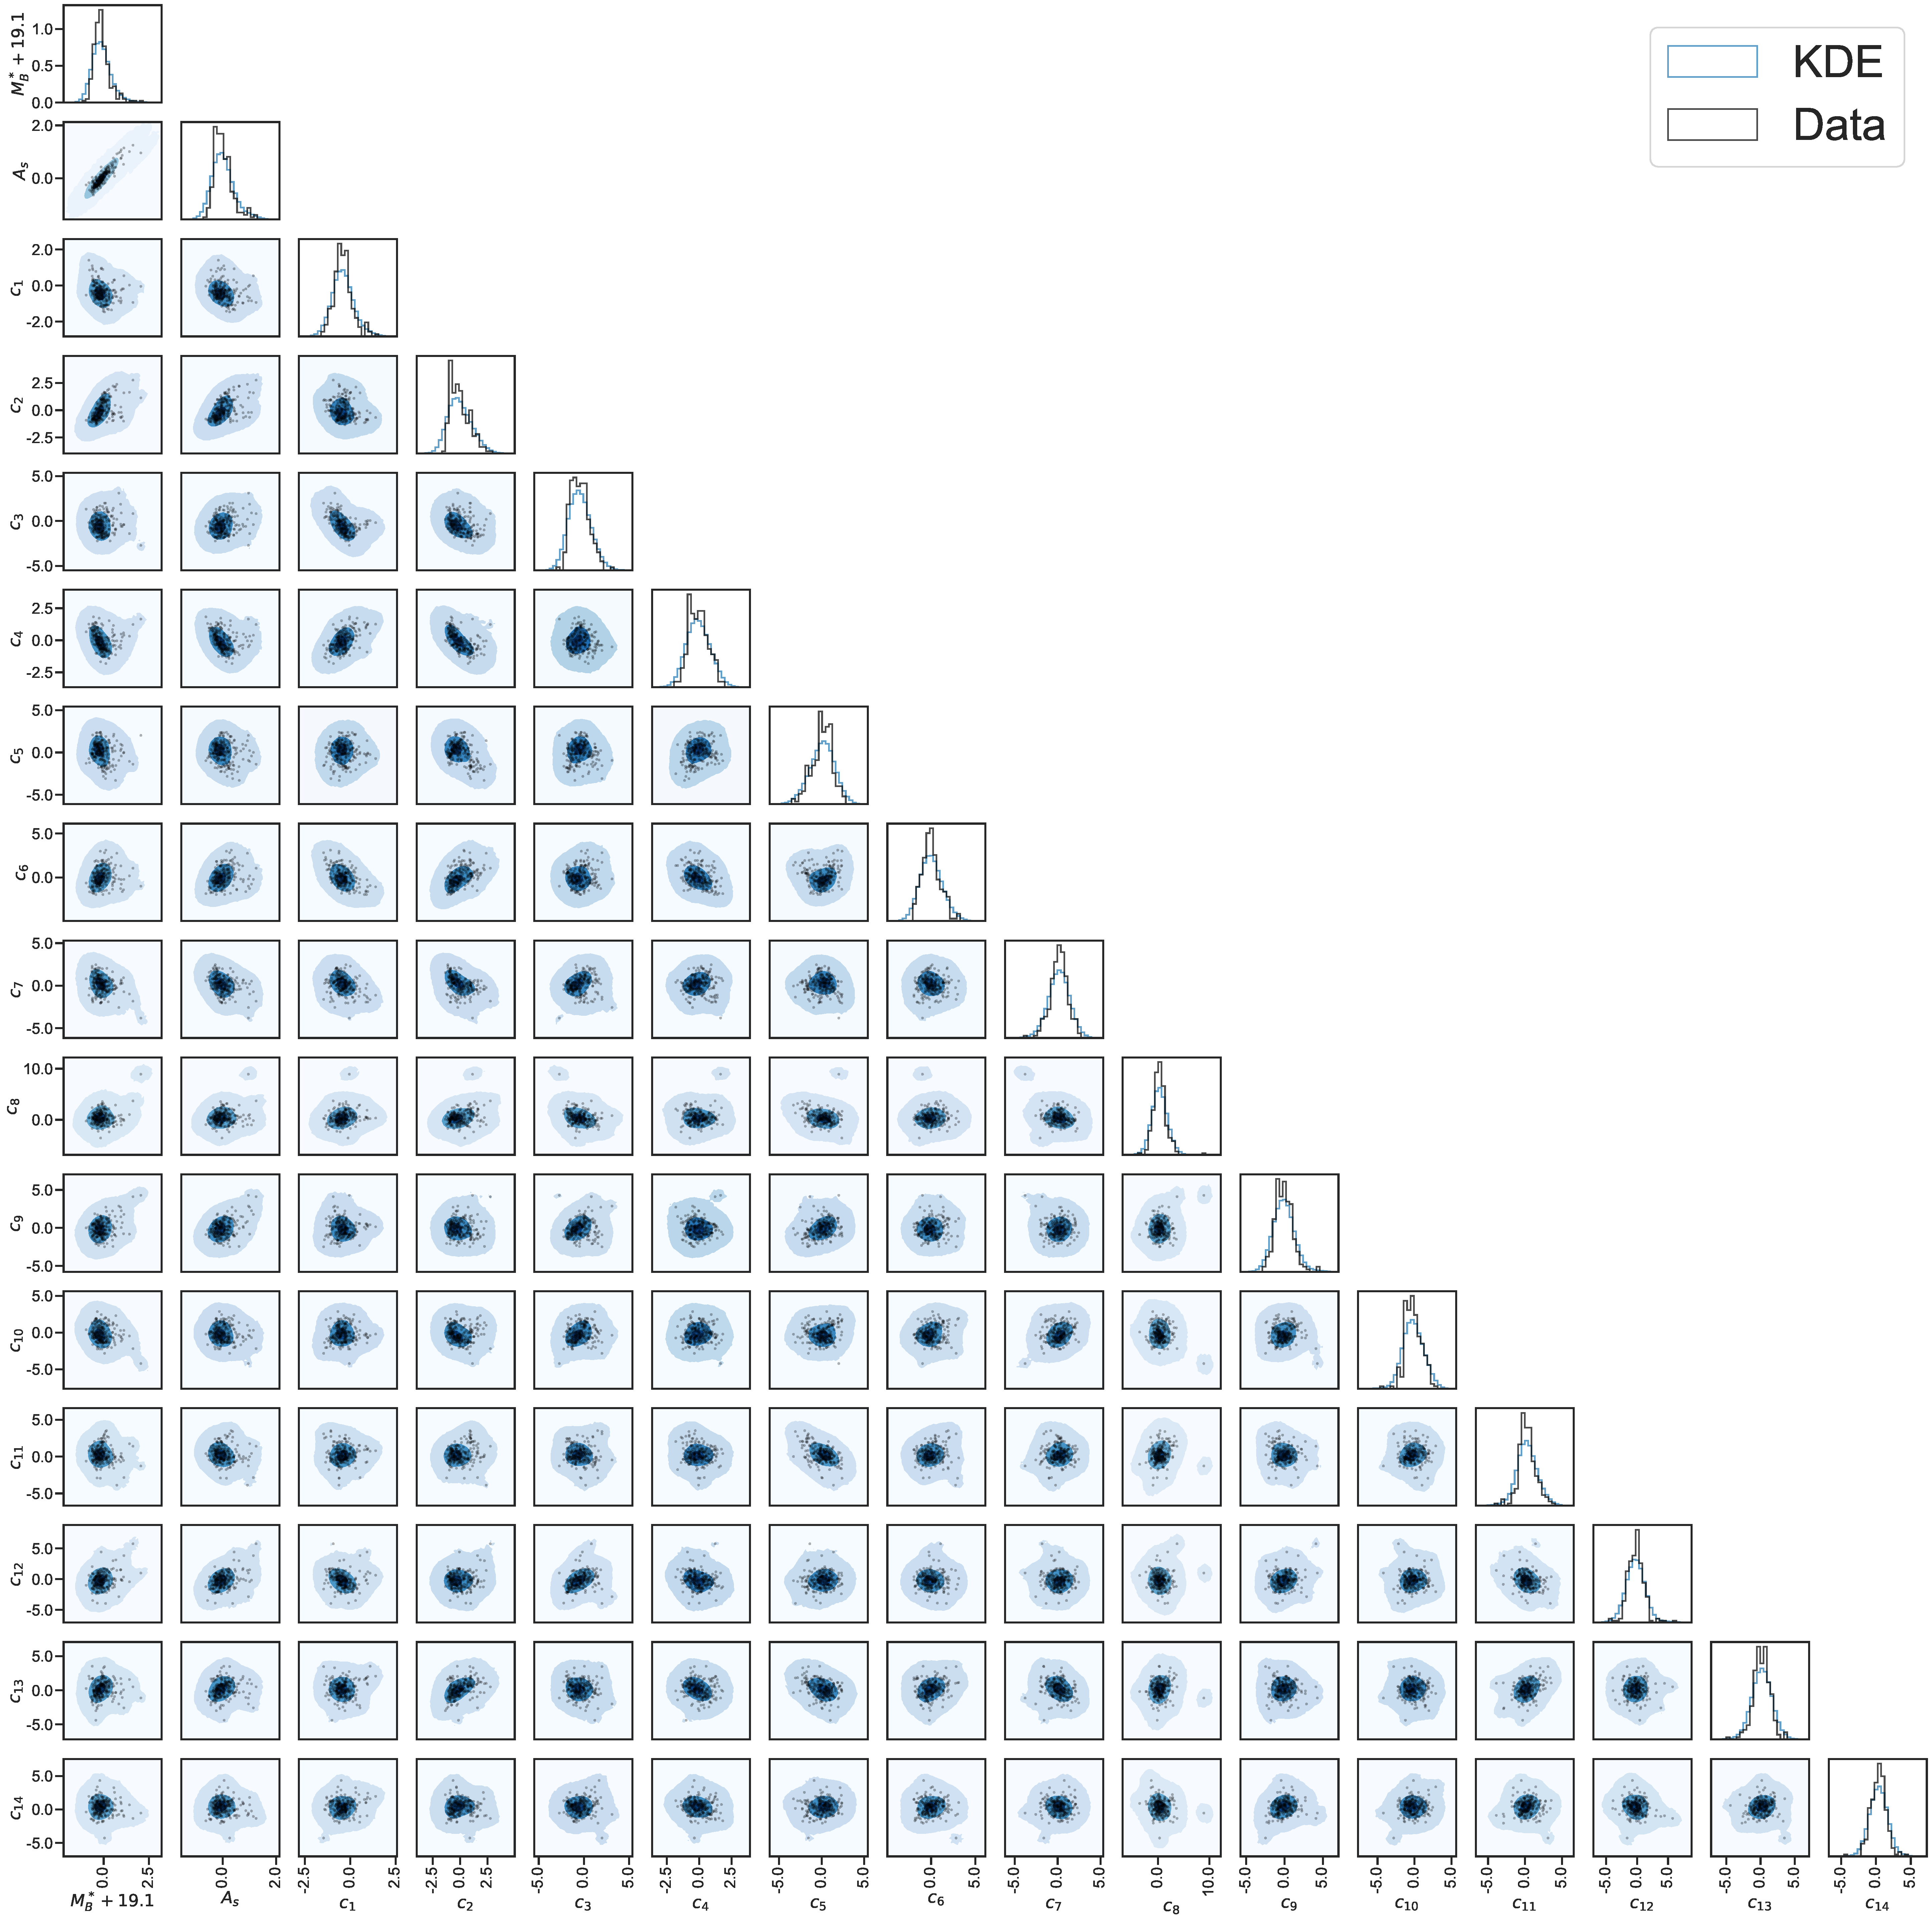
\includegraphics[width=0.9\textwidth]{figures/snemo_kde/snemo15_blob_corner.pdf}
    \caption{Same as Fig.~\ref{fig:salt2_sample}, but for SNEMO15}
    \label{fig:snemo15_sample}
\end{figure}

By eye, the marginal probability distributions of of the KDE samples appear to match the data quite well across all models. This is true even of the skewed parameter distributions, like those corresponding to the color terms in the model (SALT2 $c$ and SNEMO $A_s$). The two-dimensional marginalized distributions are also visually close to those of the data, even when the distributions deviate from a Gaussian, as they do for $c_1$ and $c_2$, for example, in SNEMO7. In Section \ref{sec:spec_diversity}, we further quantify these qualitative descriptions by comparing the distributions of spectral feature indicators from the data to the distributions obtained from spectra simulated using the KDE model and a multivariate Gaussian model of the spectral model parameters.

% Calculating this distance in many dimensions is possible, but computationally difficult because of memory limitations associated with calculating large dimensional histograms. Therefore, we chose to compare each of the \emph{marginalized} distributions of each spectral model parameter. The Cram\'{e}r distances between the spectral model parameter marginal distributions from the best-fit KDE and from the data, as well as corresponding distances where a simple multivariate Gaussian replaces the KDE, are presented in Fig.~\ref{fig:distances}.

% \begin{figure}
%     \centering
%     \includegraphics[width=0.9\textwidth]{figures/snemo_kde/cramer_distances_param_space.pdf}
%     \caption{Cram\'{e}r distances between the empirical marginal distributions functions of the data sample and samples from a multivariate Gaussian (blue) and samples from the KDE (orange) for each parameter in each of the spectral models studied.}
%     \label{fig:distances}
% \end{figure}

% In the fewer-parameter models (SNEMO2 and SALT2), the marginal distributions of the parameters found with the KDEs match those from the data much better than those drawn from a simple multivariate Gaussian. For SNEMO7, some of the marginalized parameter distributions, like $c_2$, are better described by the KDE than the Gaussian. Others, however, are better approximated by a Gaussian distribution. For SNEMO15, each of the marginalized parameter distributions are better modeled by Gaussians than they are by the marginalized KDEs. 

% It is important to note that the metric we are using uses only the information from the marginalized probability distributions, and therefore cannot account for skewness and non-Gaussianity in the joint probability distributions. As an example of this effect, we show the observed 2-dimensional joint distribution of SNEMO15 $A_s$ and $c_1$, along with contour plots of the same distribution given by the KDE and a multivariate Gaussian in Fig.~\ref{fig:snemo15_joint_example}. While the Cram\'{e}r distance between the data and the marginalized KDE distributions of these two parameters is larger than the distance between the data and the marginalized Gaussian distribution, we see visually that the KDE seems to better capture the deviations from pure Gaussianity in the joint distributions, as evidenced by the closer agreement of the modes of the distributions and incorporation of larger tails in the distribution. Moreover, we will see in Section~\ref{sec:spec_diversity} that using the KDE to model the spectral model parameter space allows us to capture a more realistic range of spectral feature measurements. The distances presented are meant to serve as a rough heuristic for the agreement between the distributions found by this technique and the data. A more detailed look, perhaps exploring the Cram\'{e}r distances in the two-dimensional distributions, is left to future work.

% \begin{figure}
%     \centering
%     \includegraphics[width=0.6\textwidth]{figures/snemo_kde/snemo15_nongaussian_example.pdf}
%     \caption{Comparison of the KDE estimate (blue filled contours representing the 68th, 95th, and 99th percentiles of samples drawn from the full 16-dimensional estimate) and multivariate Gaussian estimate (similarly spaced red line contours) of the joint probability distribution between SNEMO15 $A_s$ and $c_1$. While the Gaussian estimate shows a closer agreement in the marginal distribution of these parameters, according to the Cram\'{e}r distance (see Fig.~\ref{fig:distances}), the KDE seems to allow a wider variety of values and better captures the skewness of this data because it is not constrained to match the Gaussian form.}
%     \label{fig:snemo15_joint_example}
% \end{figure}

\subsection{Generating Mock Observations}
With the modeled latent space in hand, we can easily obtain new SN~Ia instances to use in further analyses by drawing from the underlying joint probability distribution, calculating the scaling coefficient $x_0$ or $c_0$, and plugging the resulting parameters into Eqn. \ref{eqn:salt_flux_model} or \ref{eqn:snemo_flux_model}. This process gives us a grid of flux values across the model wavelength range (3305-8685~\AA\; for the SNEMO models or 2000-9200~\AA\; for SALT2) and phase range ($-10$ to $+40$ rest-frame days after maximum brightness for the SNEMO models or $-20$ to $+50$ rest-frame days for SALT2).

As explained in Section~\ref{sec:data}, we have modeled the absolute magnitude, rather than the redshift-dependent scaling parameters $x_0$ and $c_0$. To convert the $M_B^* + 19.1$ value to $x_0$ or $c_0$, we first choose a redshift $z$ for the supernova instance based on the needs of our analysis and calculate $m_B$, the peak apparent magnitude of an object at that redshift with $c_0=1$ and all of the remaining parameters set to values determined by the draw from the modeled distribution. We also calculate the desired apparent magnitude, $m_B^*$, by adding the distance modulus $\mu(z)$ from our fiducial cosmology to the apparent magnitude $M_B^*$ drawn from the modeled distribution. The final scale factor is then given by 
$$c_0 = 10^{-0.4(m_B^*-m_B)}.$$

Once we have our grid of flux values $f_{mod}(\lambda, p)$, we can then easily synthesize spectroscopy or photometry of any resolution or signal-to-noise ratio using a tool like \verb|sncosmo|\footnote{\url{https://sncosmo.readthedocs.io/en/v2.1.x/}} \added{\citep{Barbary:11938}}. In Fig.~\ref{fig:example_prism_spec}, we show spectra of an example object at redshift $z=0.775$ with intrinsic flux determined by a draw from the KDE model of the SNEMO15 model parameters, using the spectral resolution of the proposed Roman Space Telescope prism spectrograph and signal-to-noise equivalent to an exposure time of roughly one hour. Fig.~\ref{fig:example_roman_lc} shows the same object but observed through photometry in the bandpasses proposed for the Roman Wide Field Instrument for a similar exposure time \citep{rubin_evaluating_2020, roman_space_telescope_reference_information_roman_2019}. 

\begin{figure}
    \centering
    \includegraphics[width=0.9\textwidth]{figures/snemo_kde/example_roman_spec.pdf}
    \caption{A series of synthesized spectral observations at a range of phases for a single object at redshift $z=0.775$ generated from a random draw from the SNEMO15 KDE. The resolution matches the proposed design of the Roman Space Telescope prism spectrograph, and the signal-to-noise ratio representing the level that could be obtained with an hour of exposure time. The black lines represent the underlying spectral energy distribution generated by our model, and the blue points represent the flux values in each prism wavelength bin, along with their associated errors.}
    \label{fig:example_prism_spec}
\end{figure}

\begin{figure}
    \centering
    \includegraphics[width=0.9\textwidth]{figures/snemo_kde/example_roman_lc.pdf}
    \caption{Synthetic photometry of the same object shown in Fig.~\ref{fig:example_prism_spec}, but observed photometrically in the Roman Wide Field Instrument bandpasses. Again, the lines represent the underlying flux of the generated supernova. The points represent an example of the noisy observed flux, and its associated errors.}
    \label{fig:example_roman_lc}
\end{figure}

\section{Evaluating Spectral Diversity}
\label{sec:spec_diversity}
As another means of quantifying the usefulness of this tool, as well as a concrete example of the kind of analysis that is uniquely enabled by both a non-parametric model of spectral model parameters and the use of spectral models with more degrees of freedom (i.e. SNEMO7 and SNEMO15), we compare the distributions of several spectral features measured from the training spectra to those obtained with data simulated by the techniques introduced in this work. The development of the SNEMO models was largely motivated by the recognition that spectral models like SALT2 do not capture the full range of spectral variation that is seen in Type Ia supernovae \citep{saunders_snemo_2018}. This study aims to quantify how well higher-dimensional linear models and non-parametric models of the latent parameter space of these linear models can capture the non-linear features that may provide a better understanding of supernova standardization and supernova physics.

We chose to focus on the velocities and pseudo-equivalent widths of the \CaIIHK{} doublet, the \SiIIblue line, and the \SiIIred line at maximum brightness. These spectral indicators are commonly used in studies aiming to improve the standardization of supernova brightnesses beyond light curve shape and color, or to quantitatively subclassify Type Ia supernovae in order to gain a better understanding of their physics. The ejecta velocities of SNe~Ia, measured by the line velocities of \SiIIred and \CaIIHK{}, have been shown to correlate with their intrinsic colors \citep{foley_measuring_2011, foley_velocity_2011, foley_relation_2012, mandel_type_2014}. The width of the \SiIIred line shows a similar correlation \citep{foley_velocity_2011}. All of these relationships can lead to potential redshift-dependent distance bias if left uncorrected. An example subclassification scheme using these parameters is the Branch classification scheme \citep{branch_comparative_2006}, which arranges SNe~Ia by the widths of their \SiIIblue and \SiIIred lines, showing that there is a wide range in spectral feature behavior within the Ia class. 

For the observed data, we measured these features using a method similar to \cite{blondin_using_2006}, in which we first smooth the spectrum, then define a pseudo-continuum from the local maxima near the features in question. Using the smoothed, pseudo-continuum-removed flux, we use the relativistic Doppler formula to calculate the eject velocities, and integrate the flux to find the pseudo-equivalent width. When making measurements of the spectral features from the generated spectra, we proceed similarly, but skip the smoothing step, as the spectrum is already assumed to be noiseless. Full details of this process are presented in Appendix \ref{app:spec_feat}. 

The spectral indicators were measured from the spectrum of each supernova in our data set that was closest to the SALT2-predicted time of B-band maximum brightness, $t_0$. To minimize the impact of phase evolution of the features, we remove from the analysis all objects that do not have a spectrum within $\pm 5$ rest-frame days of $t_0$. This leaves 213 supernovae. Code to perform these measurements is publicly available through the \verb|spectral_lines| package \footnote{\url{https://github.com/sam-dixon/spectral_lines}}.

\subsection{Comparing Features Measured from Data and from Best-fit Spectral Models}
We would like to separate our quantification of how well the spectral flux models themselves are able to capture the full distributions of spectral features from how closely samples generated from the KDE models of the spectral model parameters mimic the true distribution. To answer the first question, we make measurements of the spectral features from noiseless, at-max spectra synthesized directly from the best-fit spectral model parameters for each supernova and each spectral model. We will refer to these measurements as the model measurements.

Fig.~\ref{fig:model_vSi_recovery} shows histograms of the residuals between these model-measured velocity of \SiIIred{} ($v_{6355}$) and the data-measured velocity for each object in our data set. We can see that as the number of model components increases, the scatter on these residuals decreases, indicating that the increased flexibility of these higher-dimensional spectral models allows them to capture these spectral features. At SNEMO15, average difference between the model and data measurements of the velocity of this line is comparable in size to the typical measurement error of this feature.

\begin{figure}
    \centering
    \includegraphics[width=0.9\textwidth]{figures/snemo_kde/model_vSi_recovery.pdf}
    \caption{Histograms of the residuals between the velocity of the \SiIIred line as measured from the data and as measured from the spectrum generated with the best-fit spectral model parameters. Lower dimensional models (SALT2 and SNEMO2) }
    \label{fig:model_vSi_recovery}
\end{figure}

This general trend is seen across all the spectral indicators studied, with the exception of the width of the \SiIIblue line; we can see this in Fig.~\ref{fig:model_spec_feat_recovery}, where we compare the normalized median absolute deviation (NMAD)\footnote{$\text{NMAD}(\bm{x})=1.4826\;\text{median}(|\bm{x}-\text{median}(\bm{x})|)$} of the residuals between model and data spectra for each spectral indicator across spectral models. It is not immediately obvious why the width of the \SiIIblue line is captured nearly as well by SALT2 and SNEMO2 as it is by SNEMO15, but not captured by SNEMO7. It may be due to the fact that it is a relatively small feature, and therefore both more difficult to measure precisely on the data spectrum and poorly sampled in the SNEMO spectral eigenvectors. Regardless, we find that SNEMO15 is the best at capturing all of the spectral indicators that we studied.

\begin{figure}
    \centering
    \includegraphics[width=0.9\textwidth]{figures/snemo_kde/model_spec_feat_recovery.pdf}
    \caption{Normalized median absolute deviation of residuals between spectral features measured from data spectra and from spectra generated from the best-fit spectral model. In general, spectral models with more parameters more closely capture the spectral feature measurements.}
    \label{fig:model_spec_feat_recovery}
\end{figure}

\subsection{Comparing Spectral Feature Distributions}
We can also compare the distributions of the spectral indicators measured from spectra generated by the KDE to those measured from spectra in our data set. To do so, we generate 1000 noiseless, at-max spectra from the KDE model of the spectral feature parameters and the multivariate Gaussian model as explained in Section~\ref{sec:making_mocks}, and measure the same six spectral indicators (velocity and equivalent width of \SiIIred, \SiIIblue, and \CaIIHK) for each of these spectra.

The empirical cumulative distributions of the data and the KDE distributions for each of the spectral models are shown in Fig.~\ref{fig:ecdf_kde}. A similar plot, but using the multivariate Gaussian model of the spectral model parameter space, is found in Fig.~\ref{fig:ecdf_gauss}. These figures look quite similar, though we can pick out some differences (like the difference in the lower velocity portion of SNEMO15 distribution of $v_\text{\SiIIblue}$, or the differing relative fractions in each mode of the bimodal $v_\text{\CaIIHK{}}$ distributions for SNEMO15).

\begin{figure}
    \centering
    \includegraphics[width=0.9\textwidth]{figures/snemo_kde/ecdf_kde.pdf}
    \caption{Empirical cumulative distribution functions of each spectral indicator for the data set and samples from the kernel density estimate of the spectral model parameter spaces.}
    \label{fig:ecdf_kde}
\end{figure}

\begin{figure}
    \centering
    \includegraphics[width=0.9\textwidth]{figures/snemo_kde/ecdf_gauss.pdf}
    \caption{Same as Fig.~\ref{fig:ecdf_kde}, but for samples from the multivariate Gaussian estimation of each of the spectral model parameter spaces.}
    \label{fig:ecdf_gauss}
\end{figure}

% In order to quantify the advantage of using the kernel density estimate over a simpler model (e.g. a multivariate Gaussian) of the joint probability distributions of the spectral model parameters, we use the two-sample Cram\'{e}r distance \citep{cramer_composition_1928} to measure the difference between the cumulative distribution function of the data and the estimated distributions from empirical cumulative distribution functions of the samples.
% The Cram\'{e}r distance $\omega$ between a probability distribution with the empirical cumulative distribution function $F(x)$ and a second probability distribution with the empirical cumulative distribution function $G(x)$ is defined by
% \begin{equation}
%     \omega^2 = \displaystyle \int_\infty^\infty [F(x)-G(x)]^2 dx
% \end{equation}
% Smaller values indicate closer agreement between the two distributions.

% This distance metric has the advantage over other more well-known test statistics (like the Kolmogorov-Smirnov statistic) of being sensitive to differences in the shape of distributions beyond just shifts in the mean or standard deviation, particularly in the tails of the distribution. This is ideal for our task because we want our parameter space estimates to match the true distribution across all portions of parameter space.

We can quantify these differences by calculating the two-sample Cram\'{e}r distances between the distributions of the data and the distributions of the samples for each feature. The Cram\'{e}r distance $\omega$ between a probability distribution with the empirical cumulative distribution function $F(x)$ and a second probability distribution with the empirical cumulative distribution function $G(x)$ is defined by
\begin{equation}
    \omega^2 = \displaystyle \int_\infty^\infty [F(x)-G(x)]^2 dx
\end{equation}
Smaller values indicate closer agreement between the two distributions. This distance metric has the advantage over other more well-known test statistics (like the Kolmogorov-Smirnov statistic) of being sensitive to differences in the shape of distributions beyond just shifts in the global mean or standard deviation, particularly in the tails of the distribution. This is ideal for our task because we want our parameter space estimates to match the true distribution across all portions of parameter space. We can also get obtain an estimate of the error on these distances via bootstrap resampling. 

The calculated Cram\'{e}r distances between the KDE and Gaussian estimates are shown, along with the similarly calculated model-to-data distances, in Fig.~\ref{fig:cramer_spec_feat}. We see a pattern similar to Fig.~\ref{fig:model_spec_feat_recovery} in the spectral feature distribution similarity across models -- in every case, spectral models with more parameters have distributions of the spectral indicators that more closely resemble the data. Additionally, for each of the spectral models, the kernel density estimate of the model parameter distributions creates spectral feature distributions that are as or more similar to the true data distribution than the Gaussian estimates and the best-fit parameter spectra. Overall, this shows that using more flexible spectral models along with more flexible parameter space models allows for a generative model that can accurately reproduce the full range of spectral behavior for simulations.

\begin{figure}
    \centering
    \includegraphics[width=0.9\textwidth]{figures/snemo_kde/cramer_distances_spec_feats.pdf}
    \caption{Cram\'{e}r distances between spectral indicator distributions for the SNfactory data and samples from the Gaussian estimates of the SALT2 and SNEMO parameter distributions, the modeled at-max spectra for the training data, and the KDE estimates of the spectral model parameter distributions.}
    \label{fig:cramer_spec_feat}
\end{figure}

\section{Conclusions}
\label{sec:conclusions}
We have presented flexible estimates of the joint probability distributions of model parameters for the SALT2 and the SNEMO models of \cite{saunders_snemo_2018}. These estimates can be used to generate synthetic spectra and photometry in simulations that exhibit more spectral diversity than current state-of-the-art simulation techniques. This increased variety makes possible a number of different analyses, from examining the robustness of the twinning technique presented in \cite{fakhouri_improving_2015}, to evaluating spectral feature measurement techniques under different observing conditions. There are a number of spectral properties of Type Ia supernovae beyond the two-parameter light curve shape and color parameters that have been shown to ultimately effect our cosmological parameter measurements. This work presents a simulation tool that properly incorporates these variations, allowing us to properly understand their impacts for future cosmological surveys.

\chapter{Measuring Type Ia Supernova Spectral Features from Low-Resolution and Noisy Spectra Using SNEMO}

\section{}
\chapter{Biases from Non-Simultaneous Regression with Correlated Covariates in Supernova Cosmology}
\label{chap:reg_bias}

\newcommand{\sgn}{\text{sgn}}

\section{Overview} \label{sec:intro}
As discussed in Chapter \ref{chap:intro}, the process of using various properties of Type Ia supernova observations to correct their absolute magnitudes is the key to using supernovae as cosmological distance indicators. This technique was instrumental in the discovery of the accelerating expansion of the Universe \citep{perlmutter_measurements_1999, riess_observational_1998}, and continues to serve as a powerful probe of the nature of the dark energy driving this acceleration.

A common analysis method for standardizing supernova brightnesses uses the SALT2 spectral model \citep{guy_salt2_2007, betoule_improved_2014, mosher_cosmological_2014} to parametrize SN~Ia light curves. The model parameters represent an individual supernova's peak apparent brightness in the Bessell B-band ($m_B^*$), temporal width ($x_1$), and observed color ($c$). The distance modulus $\mu$ to each object $i$ at redshift $z_i$ is then modeled as a linear combination of these parameters:
\begin{equation}
    \mu_i(z_i) = m_{B\;i}^*(z_i) - M + \alpha x_{1\;i} - \beta c_i
    \label{eqn:salt_mu}
\end{equation}
Typically, we would find the values of $M$, $\alpha$, and $\beta$ by minimizing the following quantity with respect to these parameters as well as the cosmological parameters of interest:
\begin{equation}
    \chi^2 = \displaystyle\sum_{i} \frac{\mu_i(z_i; m_{B, i}^*, x_{1,i}, c_i)-\mu_\text{cosmo}(z_i; \bm{\Theta})}{\sigma_{\text{obs},i}^2+\sigma_\text{int}^2},
    \label{eqn:chi2_cosmo_diag_cov}
\end{equation}
where $\mu_\text{cosmo}(z_i;\bm{\Theta})$ is the distance modulus-redshift relation determined by the cosmological parameters $\bm{\Theta}$, and $\sigma_{\text{obs}, i}$ is the observational uncertainty of the measurements. $\sigma_\text{int}$ is the intrinsic dispersion of standardized magnitudes, usually found by iteratively calculating the value of $\sigma_\text{int}$ that ensures the minimum value of $\chi^2$ is equal to 1.\footnote{Equation \ref{eqn:chi2_cosmo_diag_cov} is equivalent to Equation \ref{eqn:chi2_cosmo_full_cov}, assuming the covariance matrix is diagonal and contains just the measurement and intrinsic error terms} This process is effectively a familiar linear regression.

The need to add an additional uncertainty term in the form of $\sigma_\text{int}$ suggests that the linear relationship between SALT2 parameters and absolute magnitude may not capture all of the variation in supernova magnitudes, or that the parametrization provided with SALT2 may not capture all of the information that is needed to fully standardize supernova magnitudes \citep{saunders_snemo_2018}. This motivates the search for other observable properties of SNe~Ia that might explain this remaining variation, as well as the use of these other properties for standardization. One way to search for such properties is to measure correlations between these properties and the Hubble residuals $\mu_i(z_i;m_B^*, x_1, c)-\mu_\text{cosmo}(z_i;\bm{\Theta})$. A number of studies \citep{kelly_hubble_2010, lampeitl_effect_2010, sullivan_dependence_2010, childress_host_2013} have observed such a correlation with the host galaxy stellar mass: supernovae in galaxies with $\log(\mathcal{M}/\mathcal{M}_\odot) > 10$ are $\sim0.1$ magnitudes brighter after standardization than supernovae in galaxies with $\log(\mathcal{M}/\mathcal{M}_\odot) < 10$. \cite{rigault_evidence_2013}, \cite{childress_ages_2014}, and \cite{rigault_confirmation_2015} show that this effect could be due to similar correlations with host galaxy age. However, the significance of some of these correlations has been debated \citep[e.g.][]{jones_reconsidering_2015, jones_should_2018}, indicating that care must be taken in making these measurements.

Reporting the size of correlations with the linear regression residuals is mathematically well-motivated if the covariate used to predict these residuals is not itself correlated with those used in the original regression (if, for example, host mass were not correlated with light curve parameters). However, if this key assumption is violated, we find ourselves in a situation referred to in the statistics and econometrics literature as multicollinearity \cite[e.g.][]{farrar_multicollinearity_1967}. Multicollinearity results in unreliable and biased estimates of effect sizes.  A related concern discussed frequently  in these fields is omitted variable bias, in which a misspecification of the regression problem results in biased estimates of the true regression parameters \citep{clarke_phantom_2005, wooldridge_introductory_2013}. Indeed, \cite{smith_first_2020} shows some evidence of these effects in supernova cosmology, by  examining the bias on the measurement of the host galaxy mass step (which in turn biases estimates on the dark energy equation-of-state parameter) due to the correlation between host galaxy mass and SALT2 $x_1$. \cite{rigault_strong_2018} has also presented two different values of the size of the luminosity difference between supernovae in environments with differing star-formation rates when measuring the step with a sequential regression versus a simultaneous regression, using the larger, simultaneously-determined effect size as their main result.

In this work, we explore and quantify the general impact of the non-simultaneous regression methodology used in some Type Ia supernova analyses on reported effect sizes for both linear and step-function residual trends when multicollinearity exists. In Section \ref{sec:toy_model}, we work through an example using a generalized two-dimensional linear regression problem with correlated covariates. In Section \ref{sec:add_step}, we analyze a similar model that includes a step function and compare the results to those obtained in the linear case. We then calculate the effect that this general mathematical model has in the particular case of measuring the host galaxy mass step using literature data of SALT2 parameters and host galaxy masses in Section \ref{sec:data_comparison}, and conclude in Section \ref{sec:conclusion} by identifying previous results that have overlooked this effect and recommending that future analyses use fully simultaneous regression techniques.

\section{Toy Model: Two-dimensional Linear Regression with Correlated Covariates} \label{sec:toy_model}
We consider the following toy model: A series of $n$ observations\footnote{Note that $x_1$ here is just the vector of observations in the first dimension and should not be confused with the $x_1$ parameter of the SALT2 model discussed  in Equation \ref{eqn:salt_mu}.} $\{(x_1^{(1)}, x_2^{(1)}), \cdots, (x_1^{(n)}, x_2^{(n)})\}$ is drawn from a two-dimensional Gaussian distribution with $\mu=(0, 0)$ and a covariance matrix given by
\begin{equation}
    \Sigma = \left(
    \begin{matrix}
        \sigma_1^2 & \rho\sigma_1\sigma_2\\
        \rho\sigma_1\sigma_2 & \sigma_2^2
    \end{matrix}
    \right)
    \label{eqn:covmat}
\end{equation}
$\sigma_1$ and $\sigma_2$ are the standard deviations of the observations in the $x_1$ and $x_2$ dimensions, respectively, and $\rho$ is the Pearson correlation coefficient between them. They are not measurement errors, but measures of the natural spread in the distributions.
We then define
\begin{equation}
    y_i=\beta_1 x_1^{(i)} + \beta_2 x_2^{(i)} + \epsilon^{(i)}
\label{eqn:linear_model}
\end{equation}
where $\beta_1$ and $\beta_2$ are the regression coefficients, and $\epsilon$ is a noise vector drawn from a univariate normal distribution $\mathcal{N}(0, \sigma_\text{int}^2+\sigma_\text{obs}^2)$. This noise vector represents a combination of the intrinsic scatter in the model, as well as the observational measurement error. We can reformulate this as a matrix equation by denoting the data matrix as $\bm{X} = (\bm{x}_1, \bm{x}_2)$ and the coefficient vector as $\bm{\beta}=(\beta_1, \beta_2)$, giving $\bm{Y}=\bm{X\beta}+\bm{\epsilon}$.

Standard simultaneous two-dimensional least-squares regression gives us the estimated coefficient vector $\bm{\hat{\beta}}$ which minimizes the square of the residuals between the values predicted by the model ($\bm{\hat{Y}} \equiv \hat{\beta}_1\bm{x}_1 + \hat{\beta}_2\bm{x}_x \equiv \bm{X}\hat{\beta}$) and the data. As we show in Appendix \ref{app:simultaneous_ols}, these estimated values are
\begin{equation}
    \bm{\hat{\beta}} = (\bm{X}^T\bm{X})^{-1}\bm{X}^T(\bm{X\beta} + \bm{\epsilon})
    \label{eqn:sim_beta_vec}
\end{equation}
Since the expectation value of $\bm{\epsilon}$ is 0 by definition, the expectation value of the recovered coefficients from simultaneous regression is identical to the coefficients ($\langle\bm{\hat{\beta}}\rangle=\bm{\beta}$) regardless of the values of the regression coefficients, the covariance matrix components, or the size of the intrinsic scatter. We also show in Appendix \ref{app:simultaneous_ols} that the standard deviation of the residuals ($\bm{r}\equiv\bm{\hat{Y}}-\bm{Y})$ is simply $\sqrt{\sigma_\text{int}^2 + \sigma_\text{obs}^2}$.

In summary, when treating this data set with a simultaneous linear regression, we are able to reliably recover both the true regression coefficients and intrinsic dispersion. Though there is some uncertainty on the values of the regression coefficients that does depend on the correlation between the covariates, this uncertainty is also inversely proportional to the number of samples fit in the regression and is therefore able to be controlled in the case where $N$ is sufficiently large (see Equation \ref{eqn:var_betahat_simultaneous} in Appendix \ref{app:simultaneous_ols}).

However, as described above, oftentimes in Type Ia supernova studies, we do not perform a full simultaneous fit of all of our regression parameters. Instead, we fit the distance modulus as a linear function of SALT2 parameters and then add a correction to these distance moduli by fitting the distance modulus residuals as a function of some other parameter. This can be thought of as being analogous to performing this multivariate linear regression one covariate at a time.

We will show that in this case, no biases are introduced if there there is no correlation between the parameters used in the first regression and second regressions (i.e. $\rho=0$). However, if there is some correlation, we find that both the regression coefficients and the estimated scatter on the residuals are biased.

We introduce the notation we will use to treat this situation in our toy example. Without loss of generality, we can first fit $\bm{Y}$ as a function of $\bm{x}_1$. The estimate of the slope will be denoted $\hat{\beta_1}^\prime$ (the prime serves to differentiate this value from the coefficient estimated from the full two-dimensional regression). The residuals of this regression will be denoted $\bm{r}_1$. We then perform a second regression, predicting the residuals of the first regression $\bm{r}_2$ as a function of $\bm{x}_2$. The slope in this case will similarly be denoted $\hat{\beta_2}^\prime$, and the residuals will be denoted by $\bm{r}_2$.

In Appendix \ref{app:non_simultaneous_ols}, we obtain the forms of the expectation values for the regression coefficients resulting from this process, finding that
\begin{equation*}
    \langle\hat{\beta}_1^\prime\rangle = \beta_1 + \frac{\beta_2\rho\sigma_2}{\sigma_1}\quad\text{and}\quad\langle\hat{\beta}_2^\prime\rangle = \beta_2 - \beta_2\rho^2.
\end{equation*}

As we can see, both slopes are biased if $\rho \neq 0$. The size of the bias on both parameters is proportional to the size of the effect and the correlation between the covariates. Additionally, we can recognize that the bias on the first slope is identical to the omitted variable bias. This is expected, as performing this first part of the non-simultaneous regression perfectly simulates the textbook situation presented to describe the omitted variable bias.

We also calculate the spread of the final residuals in Appendix \ref{app:non_simultaneous_ols}, finding
\begin{equation}
    \sigma_{\bm{r}_2}^2 = \beta_2\rho^2\sigma_2^2(1-\rho^2) + \sigma_\text{int}^2 + \sigma_\text{obs}^2
\end{equation}
The standard deviation on the residuals from this analysis, often reported as the root-mean-squared (RMS) residuals, is in fact inflated by a value that scales quadratically with the correlation between the parameters and linearly with the size of the secondary effect. This bias is maximized for a given slope when $\rho = \sqrt{1/2} \approx 0.707$.
\section{Step Function Corrections}
\label{sec:add_step}
Many common analyses used in supernova cosmology do not use a linear model to correct the Hubble diagram residuals for host mass; they use a step function, motivated by the evolution of host galaxy stellar populations with redshift.\footnote{In order to maintain the differentiability of this function, some analyses approximate a step function with a logistic function with a large growth rate.  To ease our calculations (particularly in calculating the expected covariance in Equation \ref{eqn:exp_val_abs_val}), we use the sign function. The differences between the two are negligible for our purposes.} We'll modify the toy model presented in Section \ref{sec:toy_model}, and consider instead
\begin{equation}
    y_i = \alpha x_1^{(i)} + \frac{\gamma}{2}\sgn(x_2^{(i)})
\label{eqn:linear_and_step}
\end{equation}

In the simultaneous case, the expected values of the best-fit regression coefficients $\hat{\alpha}$ and $\hat{\gamma}$ are equivalent to the true values. The proof of this is very similar to the proof for the bilinear toy model presented in Appendix \ref{app:simultaneous_ols}, so we do not present any further details here.

In Appendix \ref{app:step_func}, we have worked through the non-simultaneous case where we fit the linear relationship first, followed by the step function correction to the resulting residuals. The expectation value of the best-fit linear slope ($\hat{\alpha}^\prime$) is
\begin{equation}
    \langle\hat{\alpha}^\prime\rangle = \alpha + \frac{\gamma\rho}{\sigma_1\sqrt{2\pi}}
    \label{eqn:slope_inflation}
\end{equation}
The expected step size obtained from the residuals after correcting for the linear relationship is
\begin{equation}
    \langle\hat{\gamma}^\prime\rangle = \gamma\left(1 - \frac{2\rho^2}{\pi}\right),
    \label{eqn:step_deflation}
\end{equation}
and the spread of the remaining residuals is
\begin{equation}
    \sigma_{\bm{r}_\beta}^2 = \frac{\gamma^2\rho^2}{2\pi}\left(1-\frac{2\rho^2}{\pi}\right) + \sigma_\text{int}^2 + \sigma_\text{obs}^2
\end{equation}
So, using a step-function secondary correction gives us similar biases to the linear secondary correction. The size of the step is underestimated by a factor that scales quadratically with the correlation coefficient between covariates and linearly with the true step size. Additionally, the size of the linear correction term is overestimated by a factor that scales linearly with the step size and the correlation coefficient. Finally, the variance of the residuals after correction is inflated by a factor that scales similarly. The bias on the variance of the residuals is maximal when $\rho=\sqrt{\pi/4}\approx 0.886$.

\section{Comparison to Data}
\label{sec:data_comparison}
The remaining difference between our toy models and the actual data is that the true distributions of $x_1$, $c$, and $\mathcal{M}_\text{host}$ are not purely Gaussian. While we cannot derive closed-form relations describing the impact of non-simultaneous fitting, we can simulate these effects. In this analysis, we take published values of $x_1$, $c$, and $\log(\mathcal{M}_\text{host}/\mathcal{M}_\odot)$ from the low- and mid-redshift samples of supernovae from the first three years of the Dark Energy Survey \cite[][hereafter referred to as the Low-$z$ and DES subsamples]{abbott_first_2019}, along with the Pantheon data set \citep{scolnic_complete_2018}, which combines spectroscopically-classified supernovae from PanSTARRS supernovae \cite[PS1;][]{rest_cosmological_2014, scolnic_color_2014} with supernovae from the SuperNova Legacy Survey \cite[SNLS;][]{conley_supernova_2011, sullivan_snls3_2011} and the Sloan Digital Sky Survey \cite[SDSS;][]{frieman_sloan_2008, kessler_first-year_2009, sako_data_2018}.\footnote{The DES and Low-$z$ sample data can be downloaded at \url{https://des.ncsa.illinois.edu/releases/sn}, and the Pantheon data may be found at \url{https://archive.stsci.edu/prepds/ps1cosmo/index.html}.} Each of these data sets shows a fairly strong correlation between $x_1$ and host mass, as seen in Table \ref{tab:corr_coefs}, so we can expect to find some non-simultaneous regression biases.

\begin{table}[htbp]
    \centering
    \begin{tabular}{cccc}\toprule
        Data set & $\rho_{x_1, c}$ & $\rho_{x_1, \text{mass}}$ & $\rho_{c, \text{mass}}$\\\midrule
        DES & $-0.087$ & $-0.371$ & $0.1811$\\
        PS1 & $-0.041$ & $-0.248$ & $0.0610$\\
        SDSS & $-0.035$ & $-0.297$ & $0.0002$\\
        SNLS & $0.016$ & $-0.304$ & $0.0629$\\
        Low-$z$ & $0.130$ & $-0.347$ & $-0.1052$\\
        \bottomrule
    \end{tabular}
    \caption{Pearson correlation coefficients between SALT2 parameters and host galaxy masses (measured as $\log(\mathcal{M}_\text{host}/\mathcal{M}_\odot)$). Each data set shows a relatively strong correlation between $x_1$ and mass, indicating that biases can be introduced from non-simultaneous regression.}
    \label{tab:corr_coefs}
\end{table}

To simulate the magnitude of these effects with non-Gaussian distributions, we begin by modeling $\delta$, a quantity akin to the Hubble residuals without any corrections for the light curve shape or color parameters and assuming a fixed cosmology:
\begin{equation}
    \delta= M + \alpha x_1 + \beta c + \frac{\gamma}{2}\sgn\left[\log\left(\frac{\mathcal{M}_\text{host}}{\mathcal{M}_\odot}\right) - 10 \right] + \epsilon
\end{equation}
where $\epsilon$ is a Gaussian distributed noise vector with variance $\sigma_\text{noise}^2$. For each data set, we calculate 50 instances of $\delta$ with different noise vectors for nearly 12,000 different combinations of $\alpha$, $\beta$, $\gamma$, and $\sigma_\text{int}$ in the ranges described in Table \ref{tab:sim_ranges}. We are motivated to simulate various combinations of the regression coefficients and noise values by the toy model, which showed that each of these values is intrinsically linked to the others. The overall magnitude value $M$ was fixed to $-19.1$, as the value of this offset in our model does not affect our results. For each of these simulated data sets, we perform both the full simultaneous linear and step function fit, as well as the non-simultaneous linear fit followed by a fit of the step function to the residuals of the linear fit. Note that in both cases the linear portion of the fit is done simultaneously, as is done in typical cosmology analyses.
\begin{table}
    \centering
    \begin{tabular}{cc}
    \toprule
        Parameter & Range \\\midrule
        $\alpha$ & $(0.05, 0.25)$ \\
        $\beta$ & $(2.5, 3.5)$ \\
        $\gamma$ & $(-0.1, 0.1)$ \\
        $\sigma_\text{noise}$ & $(0, 0.2)$ \\
        \bottomrule
    \end{tabular}
    \caption{Ranges for the standardization hyperparameters used in the simulation analysis.}
    \label{tab:sim_ranges}
\end{table}

The results of these simulations are tables of true values of $\alpha$, $\beta$, and $\gamma$, simultaneous best-fit values $\hat{\alpha}$, $\hat{\beta}$, and $\hat{\gamma}$, as well has non-simultaneous best-fit values $\hat{\alpha}^\prime$, $\hat{\beta}^\prime$, and $\hat{\gamma}^\prime$, for each data set. Regardless of true parameter value, the simultaneous fit parameters all match the true parameters. However, the magnitude of the error on the non-simultaneous best-fit parameters depends on the data subset in question as well as on the true values of the parameters. The relationships are all linear, i.e.
\begin{equation}
    \gamma = c_{\gamma, 0} + \displaystyle\sum_{i\in\{\hat{\alpha}, \hat{\beta}, \hat{\gamma}\}} c_{\gamma, i}i,
    \label{eqn:lin_decomp_reg_bias}
\end{equation}
where the $c$ values are the linear coefficients relating the best-fit standardization parameters to their true values.\footnote{These coefficients are not to be confused with the SALT2 color parameter $c$ (with no subscript).} Similar relationships exist for $\alpha$ and $\beta$ as well. This is not unexpected; we see this linear relationship in our toy models as well (see Equation \ref{eqn:slope_inflation}, for example). Non-zero values of coefficients other than $c_{x, 0}$ indicate that there is ``leakage" from one standardization parameter to the other; for example, if $c_{\gamma, \alpha} \neq 0$, then the size of the $\alpha$ correction impacts the reported size of the $\gamma$ corrections. Moreover, these coefficients define a linear transformation between the true regression parameters and those coming from a non-simultaneous fit, so the inverse of these transformations can be used to correct previous non-simultaneous regressions. The transformations we obtained from our simulations are presented in Tables \ref{tab:trans_alpha}, \ref{tab:trans_beta}, and \ref{tab:trans_gamma}.

\begin{table}[htbp]
\centering
    \begin{tabular}{ccccc}\toprule
    \multirow{2}{*}{Data set} &
    \multicolumn{4}{c}{$\alpha$}\\
       {}  &  $c_{\alpha, 0}$ & $c_{\alpha,\hat{\alpha}}$ & $c_{\alpha,\hat{\beta}}$ & $c_{\alpha,\hat{\gamma}}$\\\midrule
        DES & $0.000$ & $1.000$ & $0.000$ & $0.335$\\
        PS1 & $0.000$ & $1.000$ & $0.000$ & $0.135$\\
        SDSS & $0.000$ & $1.000$ & $0.000$ & $0.125$\\
        SNLS & $0.000$ & $1.000$ & $0.000$ & $0.203$\\
        Low-$z$ & $0.000$ & $1.000$ & $0.000$ & $0.194$\\
    \bottomrule
    \end{tabular}
    \caption{Linear transformation coefficients (see Equation \ref{eqn:lin_decomp_reg_bias}) between the standardization hyperparameter $\alpha$, representing the light curve shape-luminosity correction, obtained with a non-simultaneous fit and the true values.}
    \label{tab:trans_alpha}
\end{table}

\begin{table}[htbp]
    \centering
    \begin{tabular}{ccccc}\toprule
        \multirow{2}{*}{Data set} &
        \multicolumn{4}{c}{$\beta$}\\
        {} &  $c_{\beta, 0}$ &  $c_{\beta,\hat{\alpha}}$ & $c_{\beta,\hat{\beta}}$ & $c_{\beta,\hat{\gamma}}$\\\midrule
        DES & $0.001$ & $0.000$ & $0.999$ & $-0.702$\\
        PS1 & $0.002$ & $0.000$ & $0.999$ & $-0.607$\\
        SDSS & $0.002$ & $-0.002$ & $1.000$ & $-0.134$\\
        SNLS & $0.002$ & $-0.001$ & $0.999$ & $-0.565$\\
        Low-$z$ & $0.003$ & $0.001$ & $0.999$ & $1.258$\\
    \bottomrule
    \end{tabular}
    \caption{Same as Table \ref{tab:trans_alpha}, but for the standardization hyperparameter $\beta$, representing the color-luminosity correction.}
    \label{tab:trans_beta}
\end{table}

\begin{table}[htbp]
    \centering
    \begin{tabular}{ccccc}\toprule
        \multirow{2}{*}{Data set} &
        \multicolumn{4}{c}{$\gamma$}\\
        {} &  $c_{\gamma, 0}$ &  $c_{\gamma,\hat{\alpha}}$ & $c_{\gamma,\hat{\beta}}$ & $c_{\gamma,\hat{\gamma}}$ \\\midrule
        DES & $0.000$ & $0.000$ & $0.000$ & $1.302$\\
        PS1 & $0.000$ & $0.000$ & $0.000$ & $1.111$\\
        SDSS & $0.000$ & $0.000$ & $0.000$ & $1.237$\\
        SNLS & $0.000$ & $0.000$ & $0.000$ & $1.140$\\
        Low-$z$ & $0.000$ & $0.000$ & $0.000$ & $2.072$\\
    \bottomrule
    \end{tabular}
    \caption{Same as Table \ref{tab:trans_alpha}, but for the standardization hyperparameter $\gamma$, representing the host mass-luminosity correction.}
    \label{tab:trans_gamma}
\end{table}

We can see that there is significant leakage between the size of the host mass step and the stretch and color standardization parameters $\alpha$ and $\beta$. Multiplying the coefficients relating the non-simultaneously obtained step-size by the typical size of the measured step (0.07 mag.), we can see that this leakage results in a 5--10\% error on the typical size (0.14) of the stretch parameter $\alpha$ and a $\sim$1\% error on the typical size (3.0) of the color parameter $\beta$.

More importantly, the coefficients relating the non-simultaneous step size to the true step size are greater than one for each data set. This means that by fitting the step function separately from other corrections, the true size of the step is underestimated by 10--30\%, and by a factor of two for the Low-$z$ subsample.

\section{Conclusions}
\label{sec:conclusion}
We have worked through a pedagogical example to show that performing linear regression one covariate at a time produces biased estimates of both the regression coefficients and spread of residuals when the covariates are correlated. The sizes of these biases depend directly on the magnitude of the correlation, and there are linear relationships between the error on the estimated slopes and the size of the factor that inflates the estimate of the spread of the remaining scatter. We have proven that similar relationships also hold when fitting step functions to the residuals of a linear regression (as is sometimes done in supernova cosmology) if there are correlations between the parameters being fit in each step. 

We have also presented numerical simulations based on observed data to find corrections to the biases that are introduced from non-simultaneous regression methods. Each data set studied shows the possibility of a large underestimate of the size of the host mass step regardless of values of other nuisance parameters. There are also minor biases in the model parameters governing the relationship between luminosity and light curve width (SALT2 $\alpha$) and luminosity and color (SALT2 $\beta$).

Biases are introduced when the assumptions underlying an analysis method are overlooked. In this particular case, there is an implicit assumption that all covariates must be uncorrelated in order to prevent biases from performing a two-step regression. A number of studies \citep[e.g.][]{kelly_hubble_2010, sullivan_dependence_2010, childress_host_2013, jones_reconsidering_2015, jones_should_2018, rose_think_2019, kelsey_effect_2020} have neglected this effect, leading to underestimated sizes and significances of the effect sizes they report. For the most part, cosmology analyses, \citep[e.g.][]{betoule_improved_2014, scolnic_complete_2018, smith_first_2020}, do properly account for this affect by fitting for the host mass step size simultaneously with the other standardization parameters. However, it is not yet clear if the host mass correlations are properly accounted for in the bias corrections, as discussed in \citet{smith_first_2020}. Care must be taken in presenting the size and significance of these relationships, and propagating these correlations throughout the analysis. The biases presented here can be easily avoided by fitting all nuisance parameters simultaneously when presenting measurements of the mass step.

An interactive notebook with data simulations showing the derived relationships between effect sizes and correlation coefficients for our toy model is available through Google Colab at \url{https://colab.research.google.com/drive/1p2hPC5zsZ20A8BDjH3n1Sjlb8MVi8YB2}. The data and code used for the simulations with literature data is also publicly available at \url{https://github.com/sam-dixon/sn_multicollinearity}.

\chapter{Analyzing SN Ia Spectra at Late Times}

\section{}

\printbibliography

\end{document}